\section*{Appendix Overview}
%%%%%%%%%%%%%%%%%%%%%%%%%%%%%%%%%%%%%%%%%%%%%%%%%%%%%%%%%%%
% Body
%%%%%%%%%%%%%%%%%%%%%%%%%%%%%%%%%%%%%%%%%%%%%%%%%%%%%%%%%%%
In the appendix, we provide:
 \begin{enumerate}[I]
\setlength{\itemsep}{1pt}
  \setlength{\parskip}{0pt}
  \setlength{\parsep}{0pt}
 \item - Additional analysis comparing captions and Q\&A data
 \item - Qualitative visualizations for ``What is'' questions
 \item - Human accuracy on multiple-choice questions
 \item - \change{Details on VQA baselines}
  \item - \changenew{``Age'' and ``Commonsense'' of our model}
 \item - Details on the abstract scene dataset
 \item - User interfaces used to collect the dataset
 \item - List of the top answers in the dataset
 \item - Additional examples from the VQA dataset
 \end{enumerate}

 \begin{comment}
 an update on the dataset collection in \secref{subsec:dataset_stats}, show the interfaces that were used on Amazon Mechanical Turk (AMT) in \secref{subsec:interfaces}, and show additional example questions and answers from our VQA dataset in \secref{subsec:more_examples}. Then we provide some further analysis of the VQA dataset in \secref{sec:analysis}. In addition, \secref{sec:analysis} also shows the new results of a recent experiment to estimate inter-human agreement for multiple-choice questions.
\end{comment}


%\section{VQA Dataset Collection Progress}
%\label{sec:dataset_stats}
%%%%%%%%%%%%%%%%%%%%%%%%%%%%%%%%%%%%%%%%%%%%%%%%%%%%%%%%%%%%
%
%As of this submission, the VQA dataset has 123,285 images, 215,150 questions, and a total of 430,920 answers (including answers provided by workers while looking at the image and without looking at the image; recall that the latter become options in the multiple-choice question format) for real images from the MS COCO dataset~\cite{coco}. Since the main submission, our primary focus was collecting more questions for more real images, thus the abstract scene dataset is the same size as reported in the main document.
\section*{Appendix I: Captions \vs Questions}
\label{sec:cap_vs_q}
Do questions and answers provide further information about the visual world beyond that captured by captions? One method for determining whether the information captured by questions \& answers is different from the information captured by captions is to measure some of the differences in the word distributions from the two datasets. We cast this comparison in terms of nouns, verbs, and adjectives by extracting all words from the caption data \change{(MS COCO captions for real images and captions collected by us for abstract scenes)} using the Stanford part-of-speech (POS)\footnote{Noun tags begin with NN, verb tags begin with VB, adjective tags begin with JJ, and prepositions are tagged as IN.} tagger~\cite{StanfordPOS}.  We normalize the word frequencies from captions, questions, and answers per image, and compare captions \vs questions and answers combined.  Using a Kolmogorov-Smirnov test to determine whether the underlying distributions of the two datasets differ, we find a significant difference for all three parts of speech (p $<$ .001) \change{for both real images and abstract scenes}. This helps motivate the VQA task as a way to learn information about visual scenes; although both captions and questions \& answers provide information about the visual world, they do it from different perspectives, with different underlying biases \cite{GordonVanDurme13}, and can function as complementary to one another.  %This also may help explain why performance when answering questions is significantly worse when only using the captions and not the image (\ie, Table 1 in the main paper).

%To visualize the differences between the data sets, we again use the Stanford POS tagger to tag words as nouns (NN*), verbs (VB*), adjectives (JJ*), and prepositions (IN), normalizing counts per image, and extracting the top 500 words for each.
We illustrate the similarities and differences between the word distributions in captions vs. questions \& answers as Venn-style word clouds \cite{CoppersmithKelly14} with size indicating the normalized count -- \figref{fig:noun_cloud_real} (nouns), \figref{fig:verb_cloud_real} (verbs), and \figref{fig:adj_cloud_real} (adjectives) \change{for real images and \figref{fig:noun_cloud_abs} (nouns), \figref{fig:verb_cloud_abs} (verbs), and \figref{fig:adj_cloud_abs} (adjectives) for abstract scenes}.\footnote{Visualization created using \url{http://worditout.com/}.}  The left side shows the top words in questions \& answers, the right the top words in captions, and the center the words common to both, with size indicating the harmonic mean of the counts.

We see that adjectives in captions capture some clearly visual properties discussed in previous work on vision to language \cite{MitchellEtAl13}, such as material and pattern, while the questions \& answers have more adjectives that capture what is usual (\eg, \change{``dominant'', ``approximate'', ``higher''}) and other kinds of commonsense properties (\eg, \change{``edible'', ``possible'', ``unsafe'', ``acceptable''}).  Interestingly, we see that question \& answer nouns capture information about \change{``ethnicity'' and ``hairstyle''}, while caption nouns capture information about \change{pluralized visible objects (\eg, ``cellphones'', ``daughters'') and groups (\eg, ``trio'', ``some''), among other differences.} ``Man'' and ``people'' are common in both captions and questions \& answers.

One key piece to understanding the visual world is understanding spatial relationships, and so we additionally extract spatial prepositions and plot their proportions in the captions \vs~the questions \& answers data in \figref{fig:spatial_prepositions} (left) for real images and \figref{fig:spatial_prepositions} (right) for abstract scenes.  We see that questions \& answers have a higher proportion of specific spatial relations (\ie, ``in'', ``on'') compared to captions, which have a higher proportion of general spatial relations (\ie, ``with'', \change{``near''}).

\begin{figure*}
\centering
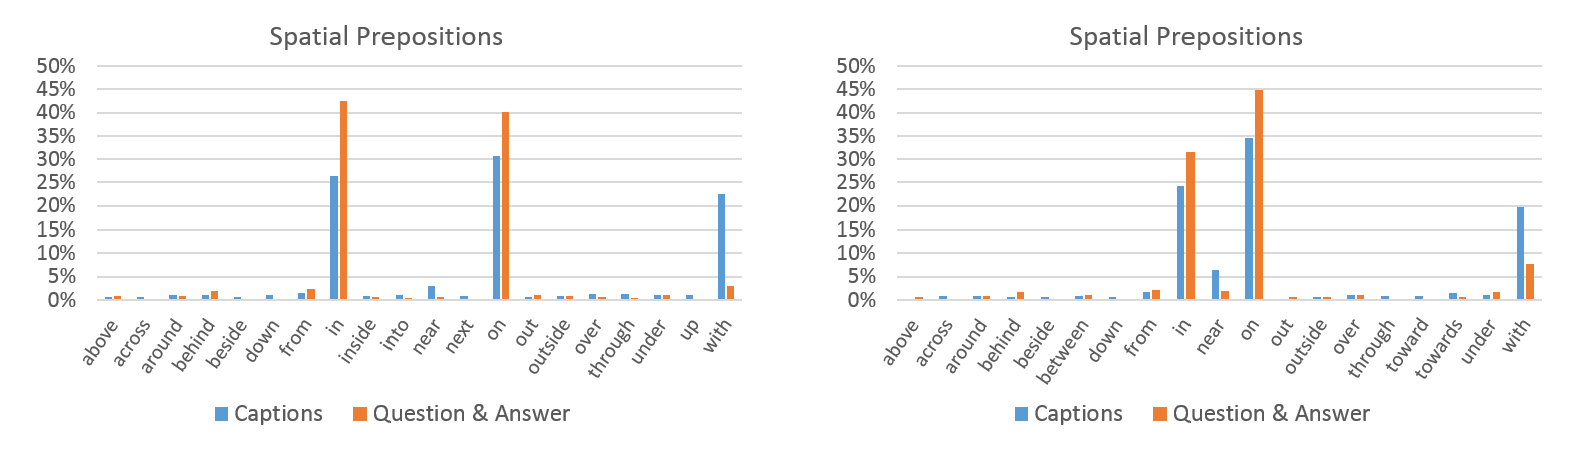
\includegraphics[width=\linewidth]{figures/spatial_prepositions.pdf}
\caption{Proportions of spatial prepositions in the captions and question \& answers for real images (left) and abstract scenes (right).}
%\vspace{-5pt}
\label{fig:spatial_prepositions}
\end{figure*}

%\begin{figure}
%\centering
%\includegraphics[width=\linewidth]{figures/coco_captions_vs_qa-spatial_prepositions.pdf}
%\caption{Proportions of spatial prepositions in the captions and question \& answers \change{for real images}.}
%%\vspace{-5pt}
%\label{fig:spatial_prepositions_real}
%\end{figure}

%\begin{figure}
%\centering
%\includegraphics[width=\linewidth]{figures/abstract_captions_vs_qa-spatial_prepositions.pdf}
%\caption{Proportions of spatial prepositions in the captions and question \& answers \change{for abstract scenes}.}
%%\vspace{-5pt}
%\label{fig:spatial_prepositions_abs}
%\end{figure}

\begin{figure*}
\centering
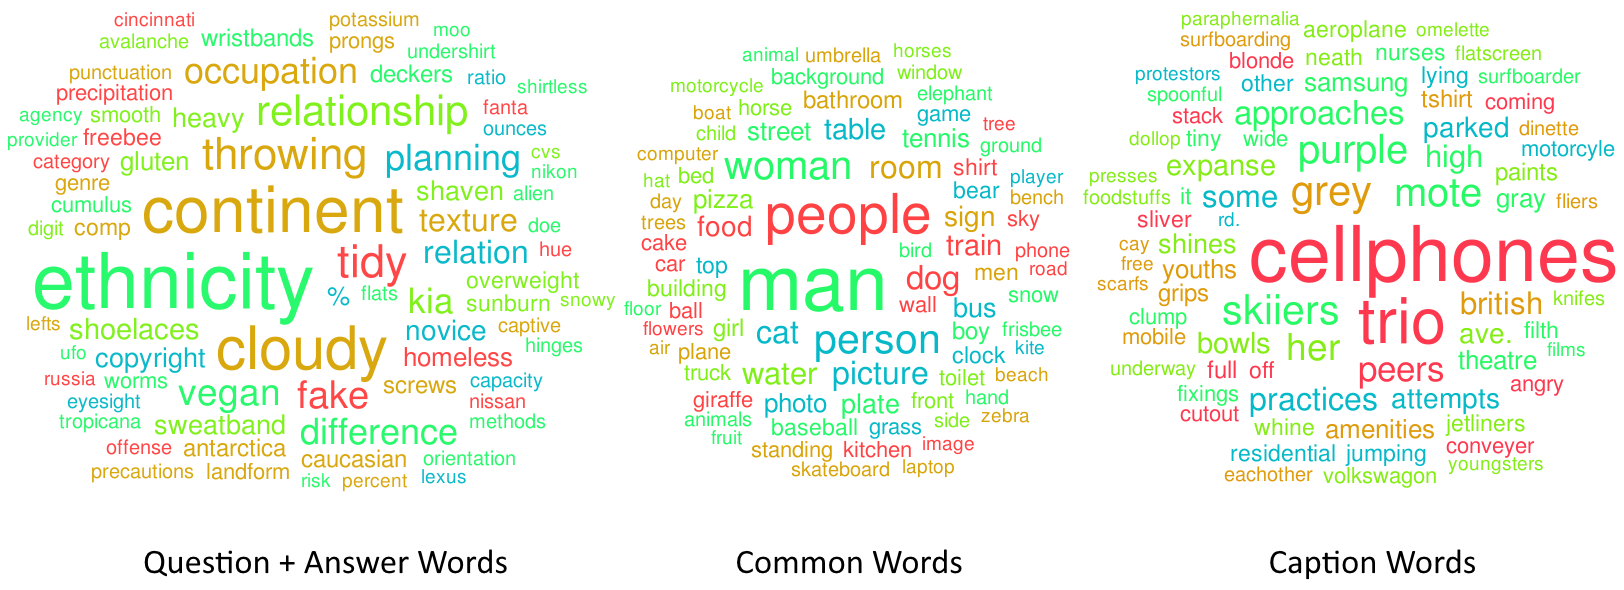
\includegraphics[width=0.9\linewidth]{figures/coco_nouns.png}
\caption{Venn-style word clouds \cite{CoppersmithKelly14} for nouns with size indicating the normalized count \change{for real images}.}
%\vspace{-5pt}
\label{fig:noun_cloud_real}
%\setlength{\belowcaptionskip}{-10pt}
\end{figure*}

\begin{figure*}
\centering
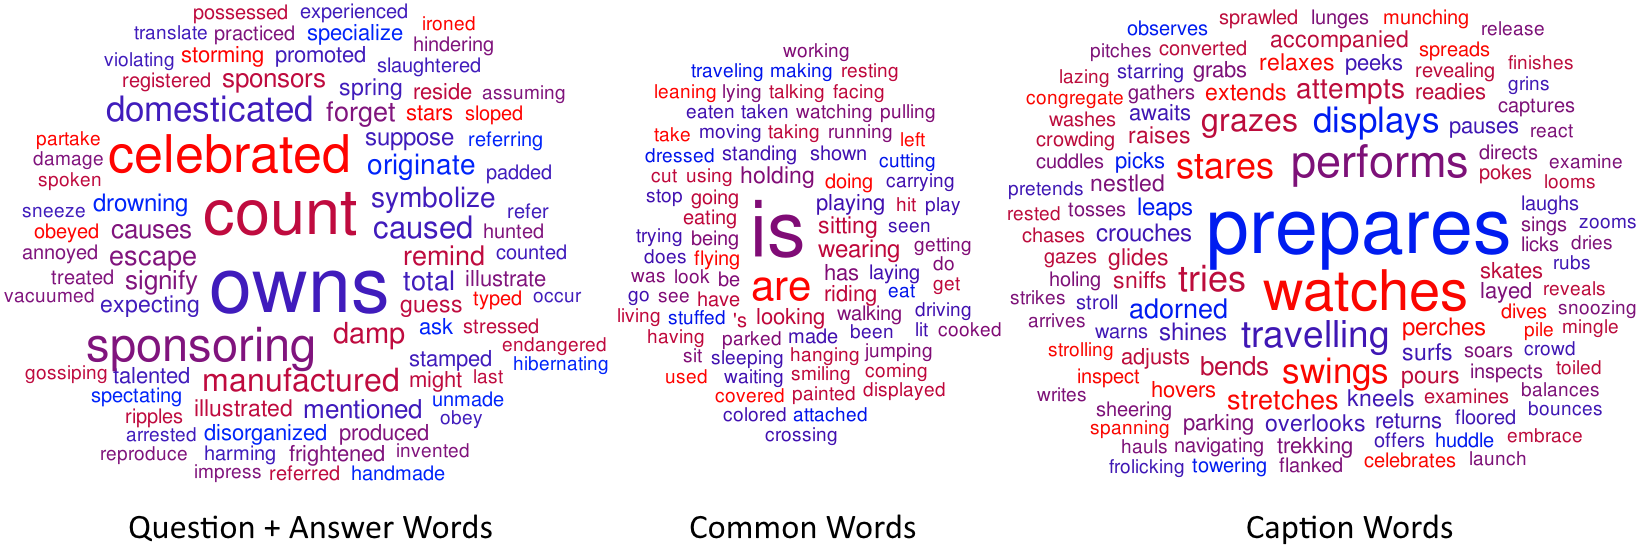
\includegraphics[width=0.9\linewidth]{figures/coco_verbs.png}
\caption{Venn-style word clouds \cite{CoppersmithKelly14} for verbs with size indicating the normalized count \change{for real images}.}
%\vspace{-5pt}
\label{fig:verb_cloud_real}
%\setlength{\belowcaptionskip}{-10pt}
\end{figure*}

\begin{figure*}
\centering
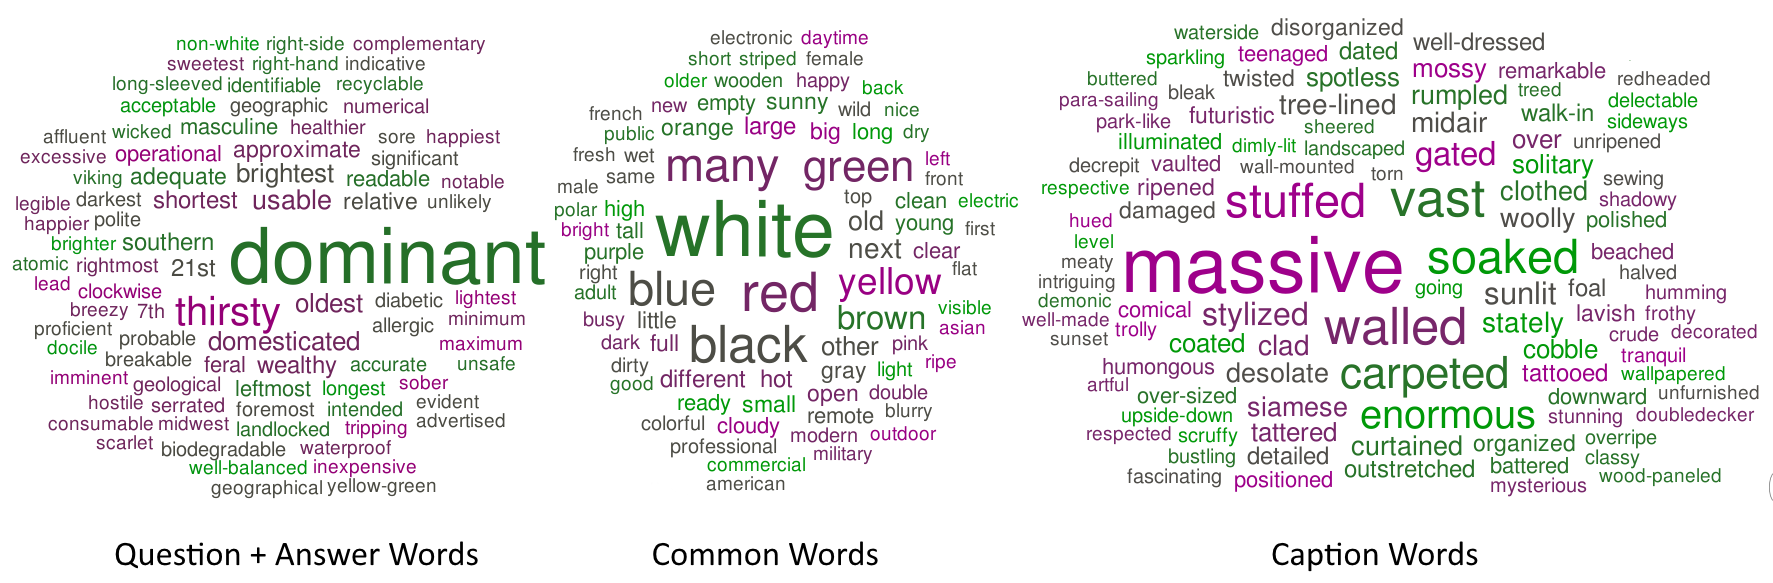
\includegraphics[width=0.9\linewidth]{figures/coco_adjectives.png}
\caption{Venn-style word clouds \cite{CoppersmithKelly14} for adjectives with size indicating the normalized count \change{for real images}.}
%\vspace{-5pt}
\label{fig:adj_cloud_real}
%\setlength{\belowcaptionskip}{-10pt}
\end{figure*}
\clearpage

\begin{figure*}
\centering
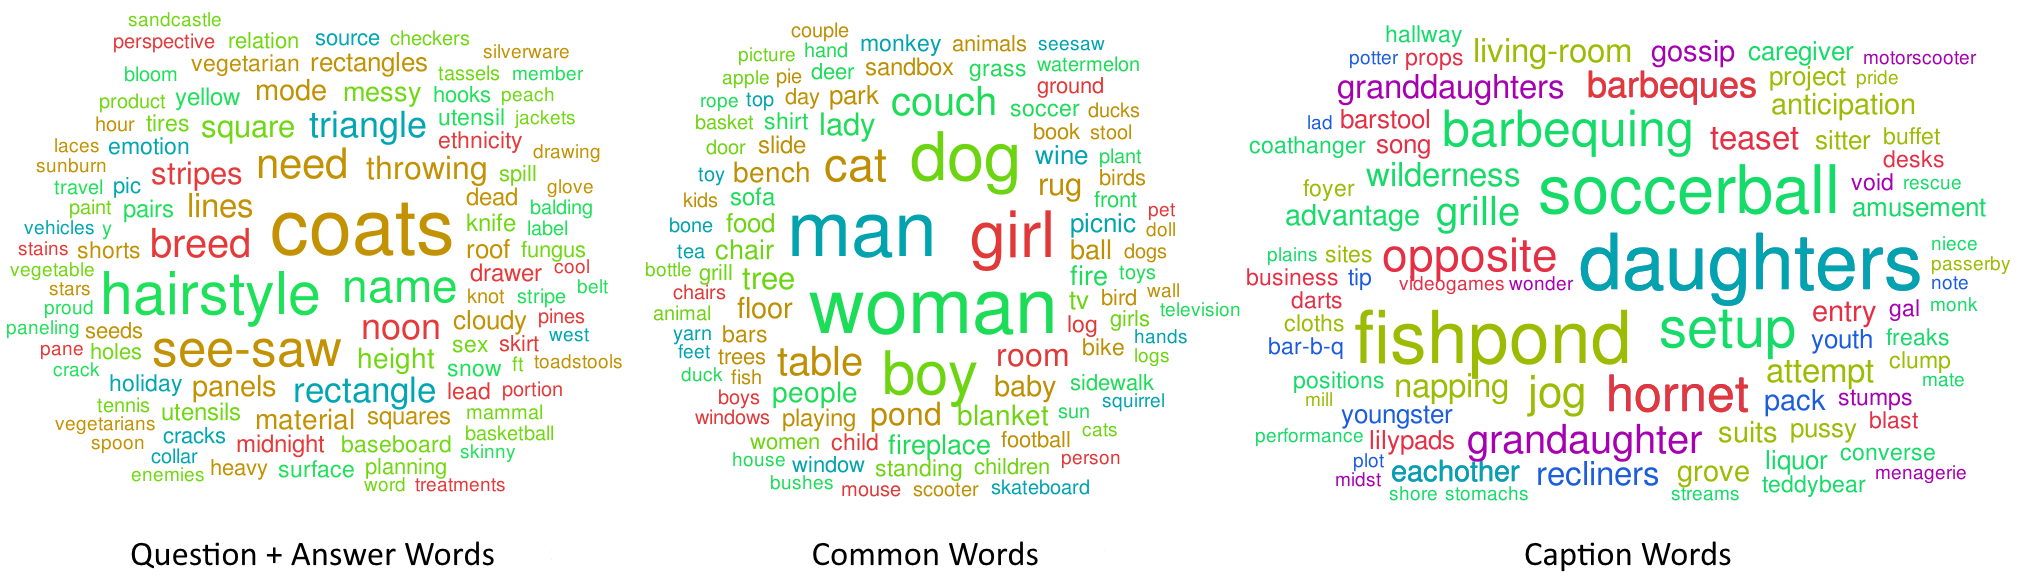
\includegraphics[width=0.9\linewidth]{figures/abstract_nouns.png}
\caption{Venn-style word clouds \cite{CoppersmithKelly14} for nouns with size indicating the normalized count \change{for abstract scenes}.}
%\vspace{-5pt}
\label{fig:noun_cloud_abs}
%\setlength{\belowcaptionskip}{-10pt}
\end{figure*}

\begin{figure*}
\centering
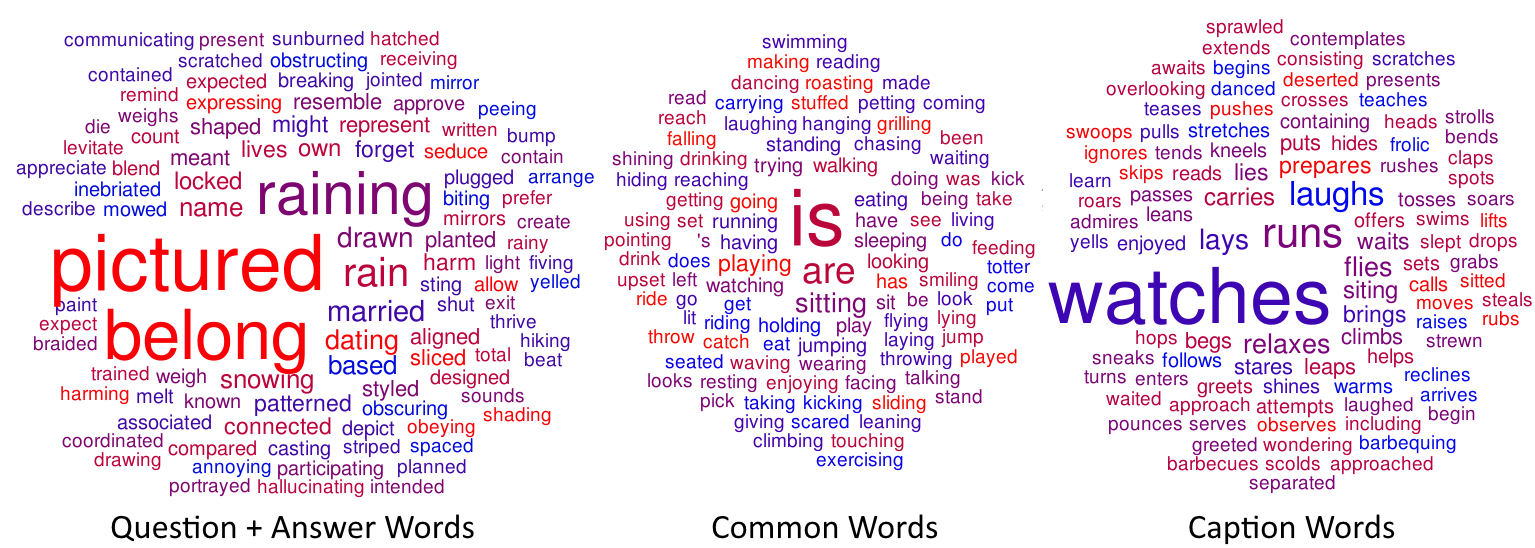
\includegraphics[width=0.9\linewidth]{figures/abstract_verbs.png}
\caption{Venn-style word clouds \cite{CoppersmithKelly14} for verbs with size indicating the normalized count \change{for abstract scenes}.}
%\vspace{-5pt}
\label{fig:verb_cloud_abs}
%\setlength{\belowcaptionskip}{-10pt}
\end{figure*}

\begin{figure*}
\centering
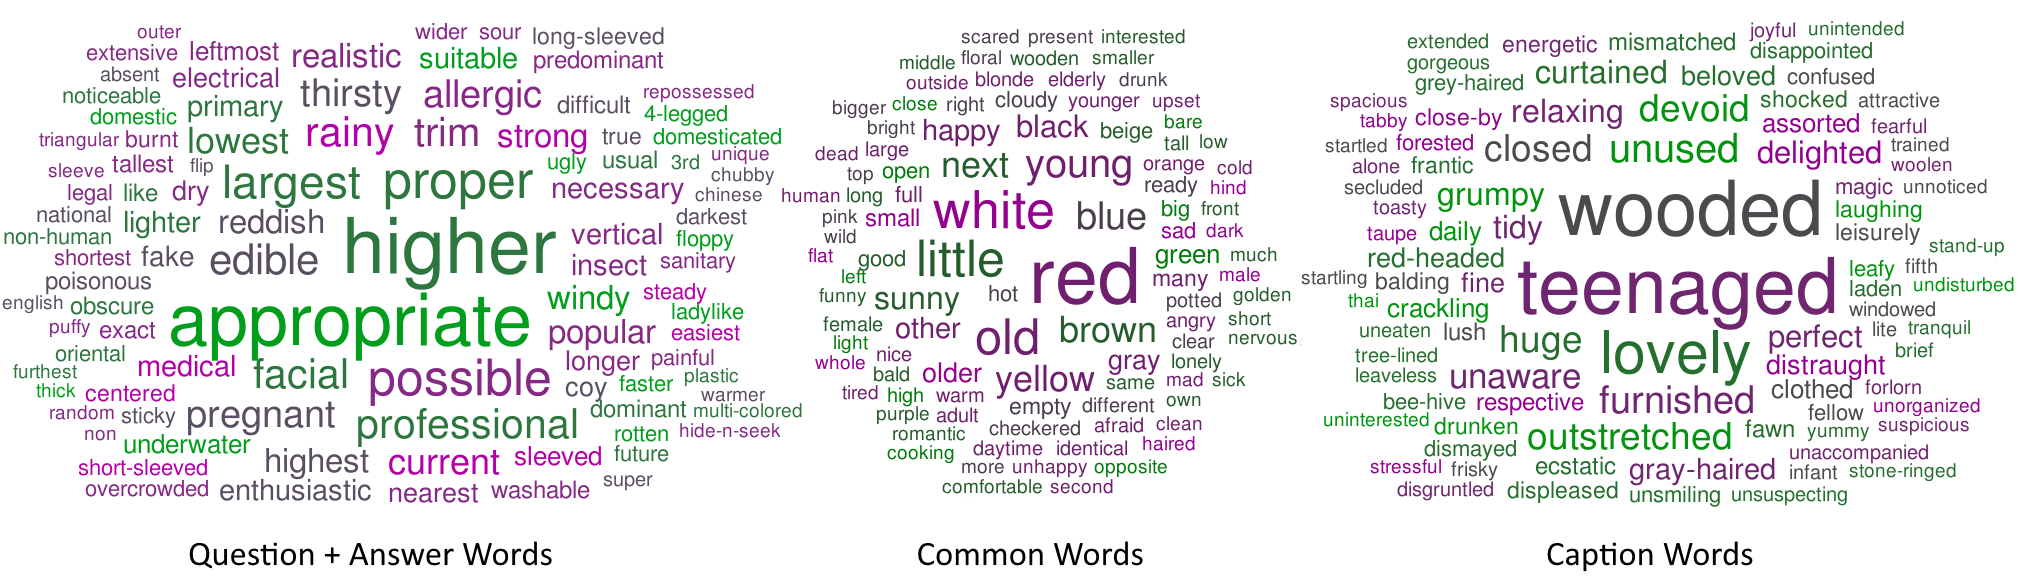
\includegraphics[width=0.9\linewidth]{figures/abstract_adjectives.png}
\caption{Venn-style word clouds \cite{CoppersmithKelly14} for adjectives with size indicating the normalized count \change{for abstract scenes}.}
%\vspace{-5pt}
\label{fig:adj_cloud_abs}
%\setlength{\belowcaptionskip}{-10pt}
\end{figure*}
\clearpage

\begin{figure*}
\centering
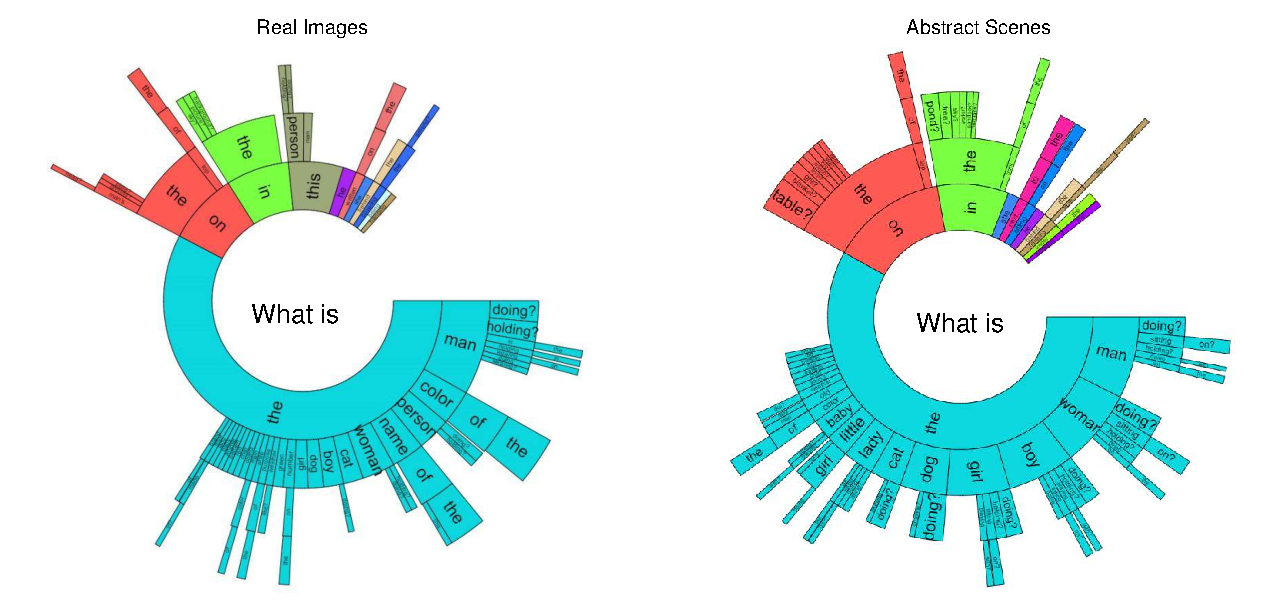
\includegraphics[width=0.95\linewidth]{figures/WhatIsQuestionTypes_mod_compressed.pdf}
\caption{\change{Distribution of questions starting with ``What is'' by their first five words for a random sample of 60K questions for real images (left) and all questions for abstract scenes (right). The ordering of the words starts towards the center and radiates outwards. The arc length is proportional to the number of questions containing the word. White areas are words with contributions too small to show.}}
%\vspace{-5pt}
\label{fig:WhatIsDistribution}
%\setlength{\belowcaptionskip}{-10pt}
\end{figure*}
\begin{figure*}
\centering
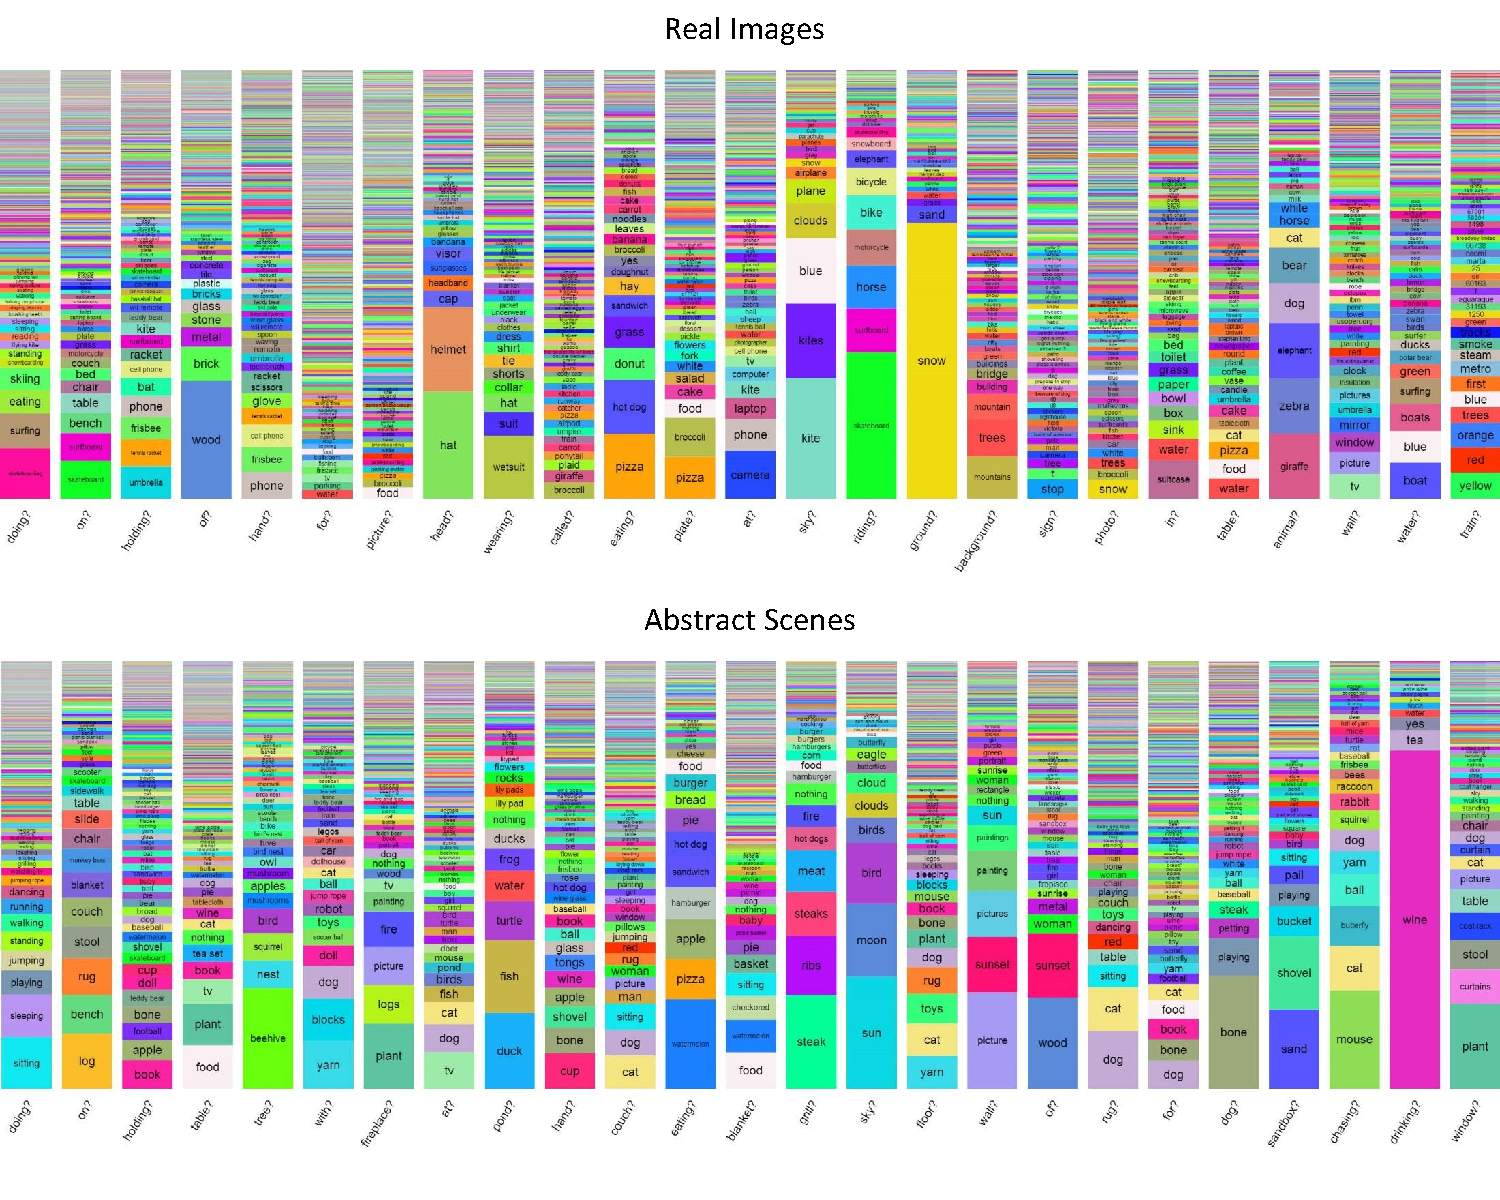
\includegraphics[width=0.95\linewidth]{figures/WhatIsAnswers-compressed.pdf}
\caption{\change{Distribution of answers for questions starting with ``What is'' for a random sample of 60K questions for real images (top) and all questions for abstract scenes (bottom). Each column corresponds to questions ending in different words, such as ``doing?'', ``on?'', \etc.}}
%\vspace{-5pt}
\label{fig:WhatIsAnswers}
%\setlength{\belowcaptionskip}{-10pt}
\end{figure*}
\section*{Appendix II: ``What is'' Analysis}
\label{sec:what_is}

In \figref{fig:WhatIsDistribution}, we show the distribution of questions starting with ``What is'' by their first five words for \change{both real images and abstract scenes}. Note the diversity of objects referenced in the questions, as well as, the relations between objects, such as ``holding'' and \change{``sitting on''}. In \figref{fig:WhatIsAnswers}, we show the distribution of answers for ``What is'' questions ending in different words. For instance, questions ending in ``eating'' have answers such as ``pizza'',  \change{``watermelon'' and ``hot dog''}. Notice the diversity in answers for some questions, such as those that end with ``for?'' or \change{``picture?''}. Other questions result in intuitive responses, such as ``holding?'' and the response ``umbrella''.

\section*{Appendix III: Multiple-Choice Human Accuracy}
\label{sec:human_mc}

To compute human accuracy for multiple-choice questions, we collected \change{three} human answers per question on a random subset of 3,000 questions \change{for both real images and abstract scenes.} In \tableref{table:humanacc_mc}, we show the human accuracies for multiple choice questions. \tableref{table:humanacc_mc} also shows the inter-human agreement for open-ended answer task. In comparison to open-ended answer, the multiple-choice accuracies are %slightly better ($\approx1\%$ increase) 
\change{more or less same}
for ``yes/no'' questions and significantly better \change{($\approx15\%$ increase for real images and $\approx11\%$ increase for abstract scenes)} for ``other'' questions. Since ``other'' questions may be ambiguous, the increase in accuracy using multiple choice is not surprising. 
%We found that \change{$\approx96\%$} of the time the majority vote response was one of the the ground truth options for both real images and abstract scenes.

\begin{table}[t]
\setlength{\tabcolsep}{3pt}
{\small
\begin{center}
\begin{tabular}{@{}llcccc@{}}
\toprule
Dataset & Accuracy Metric & All & Yes/No & Number & Other \\
%\hline
\midrule
%    & Question & 25.46 & 53.89 & 13.58 \\
%Real   & Question + Caption* & 38.28 & 63.87  & 26.90 \\
 		& MC majority vote & \change{91.54} & \change{97.40} & \change{86.97} & \change{87.91} \\
  Real  & MC average & \change{88.53} & \change{94.40} & \change{84.99} & \change{84.64} \\
     	& \changenew{Open-Ended} & \changenew{80.62} & \changenew{94.78} & \changenew{78.46} & \changenew{69.69} \\
    \midrule
    	& MC majority vote & \change{93.57} & \change{97.78} & \change{96.71} & \change{88.73} \\ Abstract & MC average & \change{90.40} & \change{94.59} & \change{94.36} & \change{85.32} \\ 
    	& \changenew{Open-Ended} & \changenew{85.66} & \changenew{95.32} & \changenew{94.17} & \changenew{74.12} \\

%for abstract    
%Majority vote across responses & \change{93.57} & \change{97.78} & \change{96.71} & \change{88.73} \\ second last column is for number questions
%Average across responses & \change{90.40} & \change{94.59} & \change{94.36} & \change{85.32} \\    
    
%\hline
%\midrule
% & Question & 31.96 & 57.10 & 15.29 \\
%Abstract %& Question + Caption & ? & ? & ? \\
% & Question + Image & 66.67 & 81.38 & 55.17 \\
\bottomrule
\end{tabular}
\end{center}
}
%\vspace{-3pt}
\caption {\changenew{For each of the two datasets, real and abstract, first two rows are the human accuracies for multiple-choice questions when subjects were shown both the image and the question. Majority vote means we consider the answer picked by majority of the three subjects to be the predicted answer by humans and compute accuracy of that answer for each question. Average means we compute the accuracy of each of the answers picked by the subjects and record their average for each question. The last row is the inter-human agreement for open-ended answers task when subjects were shown both the image and the question. All accuracies are evaluated on a random subset of 3000 questions.}}
\label{table:humanacc_mc}
%\vspace{\captionReduceBot}
\end{table}
%\begin{table}[t]
%\setlength{\tabcolsep}{5pt}
%{\small
%\begin{center}
%\begin{tabular}{@{}llcccc@{}}
%\toprule
%Dataset & All & Yes/No & Number & Other \\
%%\hline
%\midrule
%%    & Question & 25.46 & 53.89 & 13.58 \\
%%Real   & Question + Caption* & 38.28 & 63.87  & 26.90 \\
%     Real & \change{80.62} & \change{94.78} & \change{78.46} & \change{69.69} \\
%	Abstract & \change{85.66} & \change{95.32} & \change{94.17} & \change{74.12} \\
%%\hline
%%\midrule
%% & Question & 31.96 & 57.10 & 15.29 \\
%%Abstract %& Question + Caption & ? & ? & ? \\
%% & Question + Image & 66.67 & 81.38 & 55.17 \\
%\bottomrule
%\end{tabular}
%\end{center}
%}
%\vspace{-3pt}
%\caption {Inter-human agreement for open-ended answers task when subjects were shown both the image and the question.}
%\label{table:humanacc_open}
%%\vspace{\captionReduceBot}
%\end{table}

\section*{Appendix IV: Details on VQA baselines}
\label{sec:baselines}
\textbf{``per Q-type prior'' baseline.} We decide on different question types based on first few words of questions in the real images training set and ensure that each question type has at least 30 questions in the training dataset. The most popular answer for each question type is also computed on real images training set. 

\textbf{``nearest neighbor'' baseline.} For every question in the VQA test-standard set, we find its $k$ nearest neighbor questions in the training set using cosine similarity in Skip-Thought \cite{kiros2015skip} feature space. We also experimented with bag of words and Word2Vec \cite{word2vec} feature spaces but we obtained the best performance with Skip-Thought. In this set of $k$ questions and their associated images, we find the image which is most similar to the query image using cosine similarity in fc7 feature space. We use the fc7 features from the caffenet model in BVLC Caffe \cite{jia2014caffe}. The most common ground truth answer of this most similar image and question pair is the predicted answer for the query image and question pair. We pick $k = 4$ on the test-dev set.

\section*{Appendix V: ``Age'' and ``Commonsense'' of our model}
\label{sec:model_age}
We estimate the age and degree of commonsense of our \textbf{best model} (deeper LSTM Q + norm I), selected using VQA test-dev accuracies). To estimate the age, we compute a weighted average of the average age per question, weighted by the accuracy of the model's predicted answer for that question, on the subset of questions in the VQA validation set for which we have age annotations (how old a human needs to be to answer the question correctly). To estimate the degree of commonsense, we compute a weighted average of the average degree of commonsense per question, weighted by the accuracy of the model's predicted answer for that question, on the subset of questions in the VQA validation set for which we have commonsense annotations (whether the question requires commonsense to answer it).
%\arxiv{Average age and average degree of commonsense per question is computed by averaging the age and commonsense (binary response scaled to 0-100) annotations across 10 subjects for each question, respectively.} 

%\arxiv{Our model performs as well as a $4.74$ year old child (the ground-truth average age is $8.98$) and has average commonsense of $17.35\%$ (the ground-truth average commonsense is $31.23\%$)}! Again, this estimate reflects the age perceived by MTurk workers that would be required to answer the question.

\section*{Appendix VI: Abstract Scenes Dataset}
\label{sec:abstract_scenes}
In \figref{fig:clipart_details} (left), we show a subset of the objects that are present in the abstract scenes dataset. For more examples of the scenes generated, please see \figref{fig:abstract_more_examples}. The user interface used to create the scenes is shown in \figref{fig:clipart_details} (right). Subjects used a drag-and-drop interface to create the scenes. Each object could be flipped horizontally and scaled. The scale of the object determined the rendering order of the objects. Many objects have different attributes corresponding to different poses or types. Most animals have five different discrete poses. Humans have eight discrete expressions and their poses may be continuously adjusted using a ``paperdoll'' model \cite{Antol2014}.

\begin{figure*}[h]
\centering
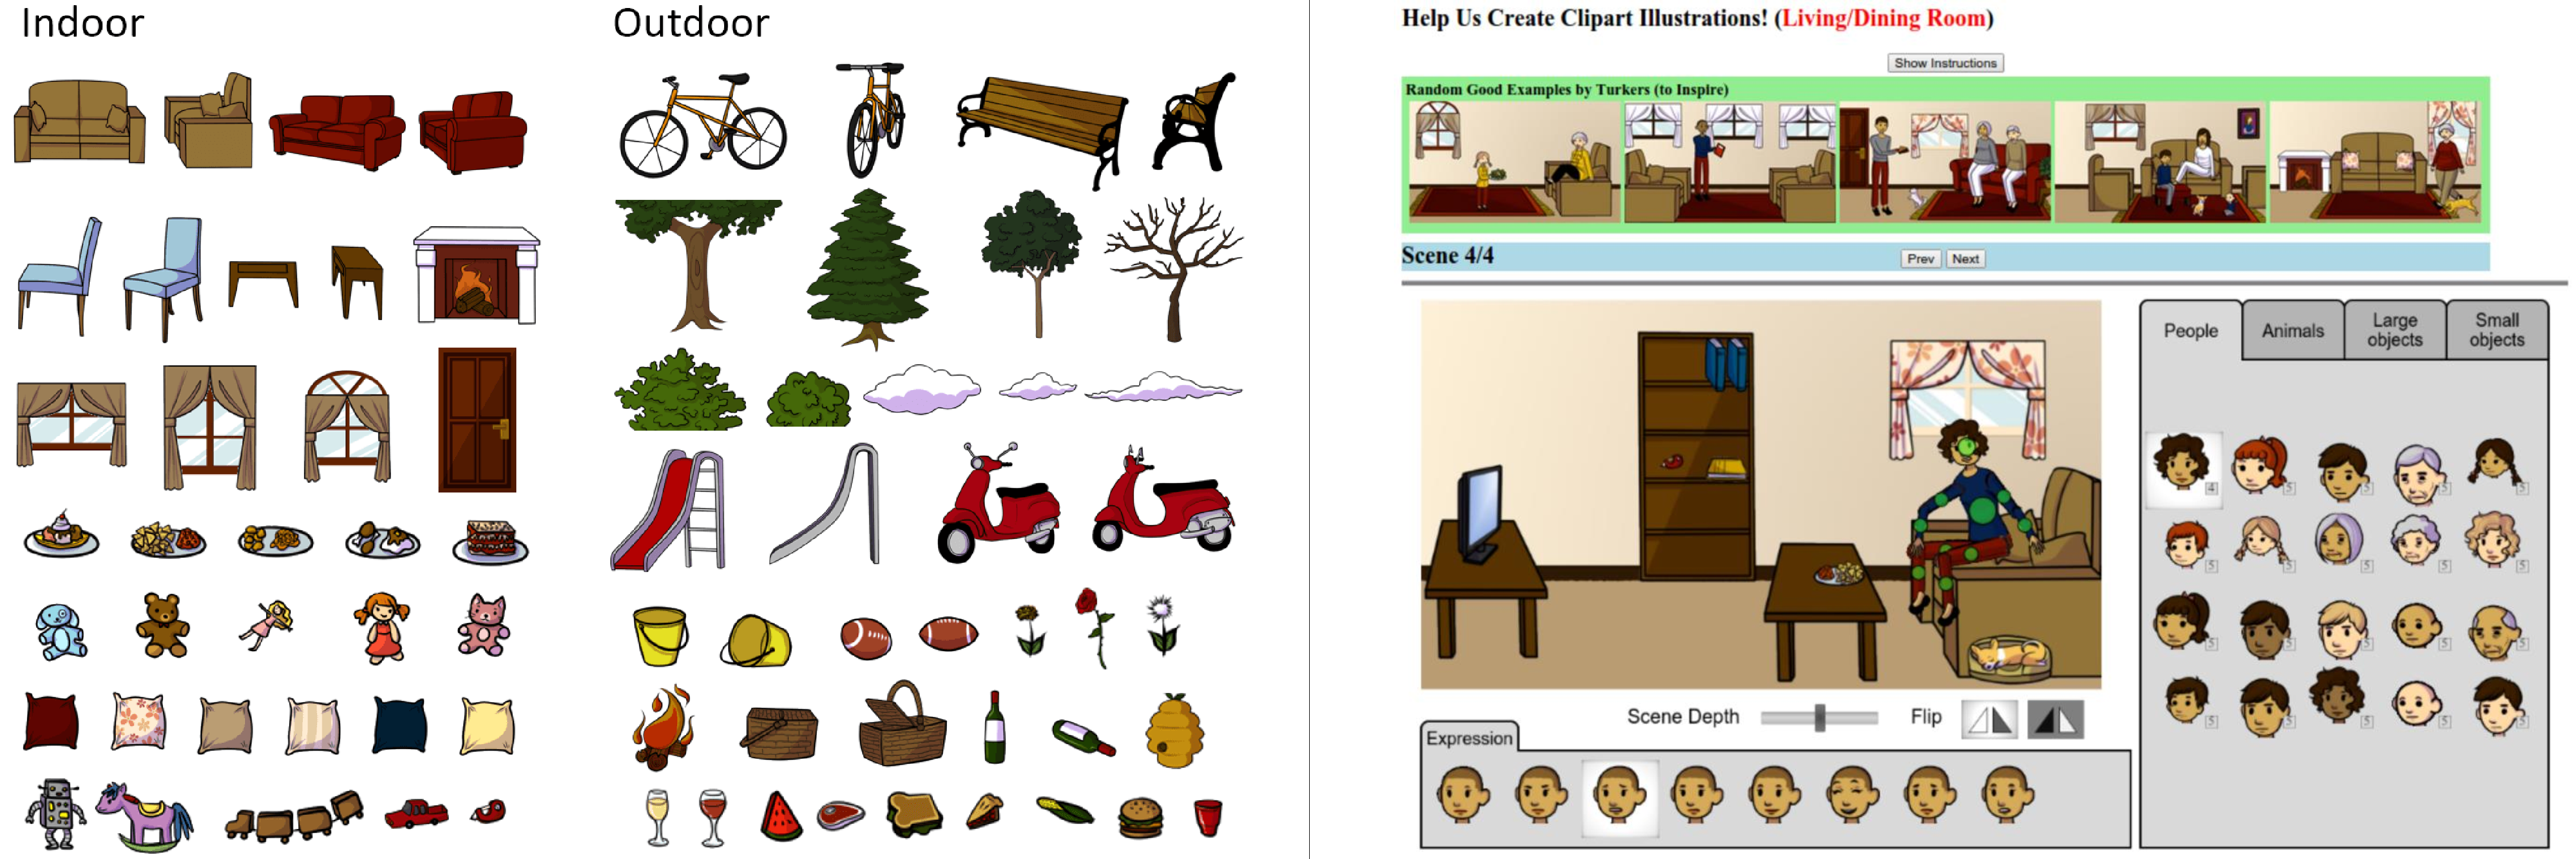
\includegraphics[width=1\linewidth]{figures/clipart_details.pdf}
\caption{Left: A small subset of the objects present in the abstract scene dataset. Right: The AMT interface for collecting abstract scenes.
The light green circles indicate where users can select to manipulate a person's pose. Different objects may be added to the scene using the folders to the right.}
\label{fig:clipart_details}
%\setlength{\belowcaptionskip}{-10pt}
\vspace{10pt}
\end{figure*}

%\begin{figure}[h!]
%\centering
%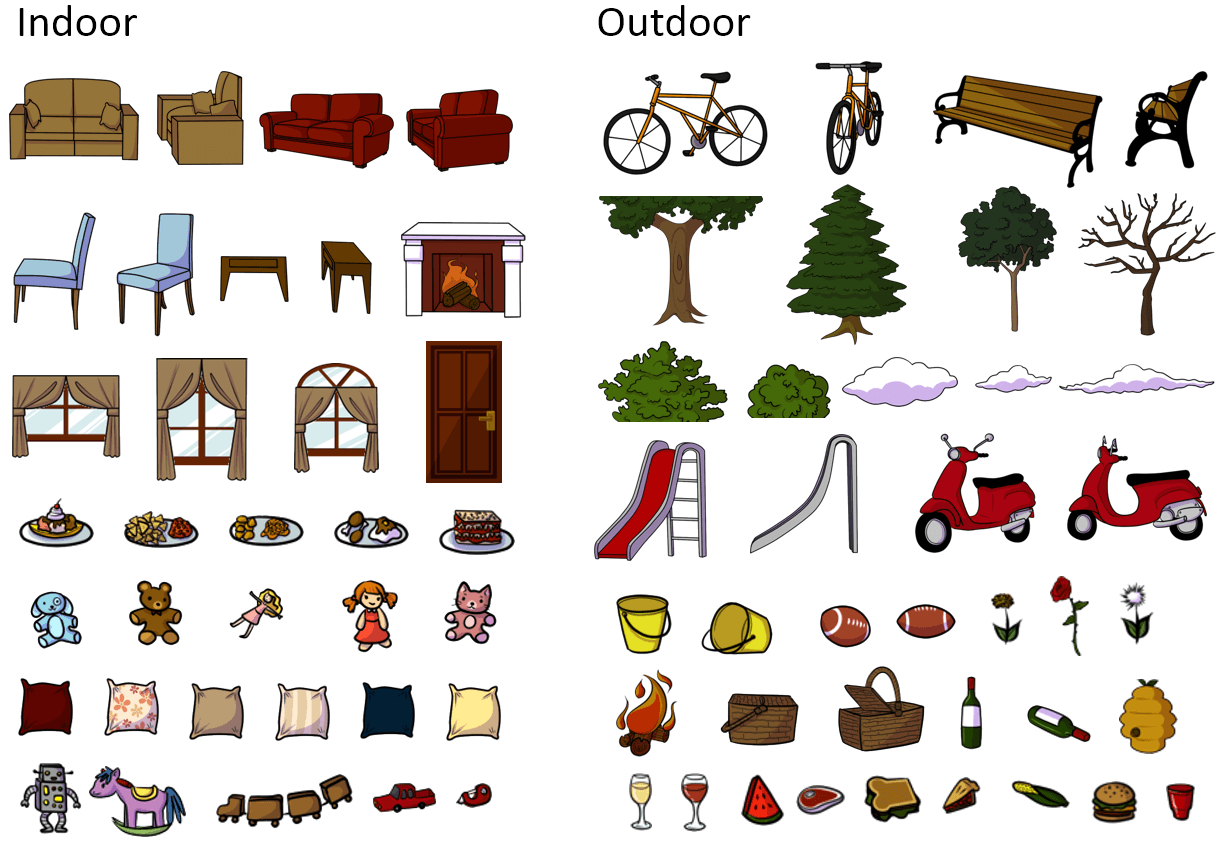
\includegraphics[width=1\linewidth]{figures/objects_min.png}
%\caption{A small subset of the objects present in the abstract scene dataset.}
%%\vspace{-5pt}
%\label{fig:abstractobjects}
%%\setlength{\belowcaptionskip}{-10pt}
%\end{figure}

%\begin{figure}[h!]
%\centering
%\includegraphics[width=1\linewidth]{figures/clipart_interface.pdf}
%\caption{The AMT interface for collecting abstract scenes.
%The light green circles indicate where users can select to manipulate a person's pose. Different objects may be added to the scene using the folders to the right.}
%%\vspace{-5pt}
%\label{fig:abstract}
%%\setlength{\belowcaptionskip}{-10pt}
%\end{figure}
\section*{Appendix VII: User Interfaces}
\label{sec:uis}
In \figref{fig:qstage03}, we show the AMT interface that we used to collect questions for images. Note that we tell the workers that the robot already knows the answer to the previously asked question(s), inspiring them to ask different kinds of questions, thereby increasing the diversity of our dataset.

\figref{fig:answimage} shows the AMT interface used for collecting answers to the previously collected questions when subjects were shown the corresponding images. \figref{fig:answoimage} shows the interface that was used to collect answers to questions when subjects were not shown the corresponding image (\ie, to help in gathering incorrect, but plausible, answers for the multiple-choice task and to assess how accurately the questions can be answered using common sense knowledge alone).

\begin{figure*}[h]
\centering
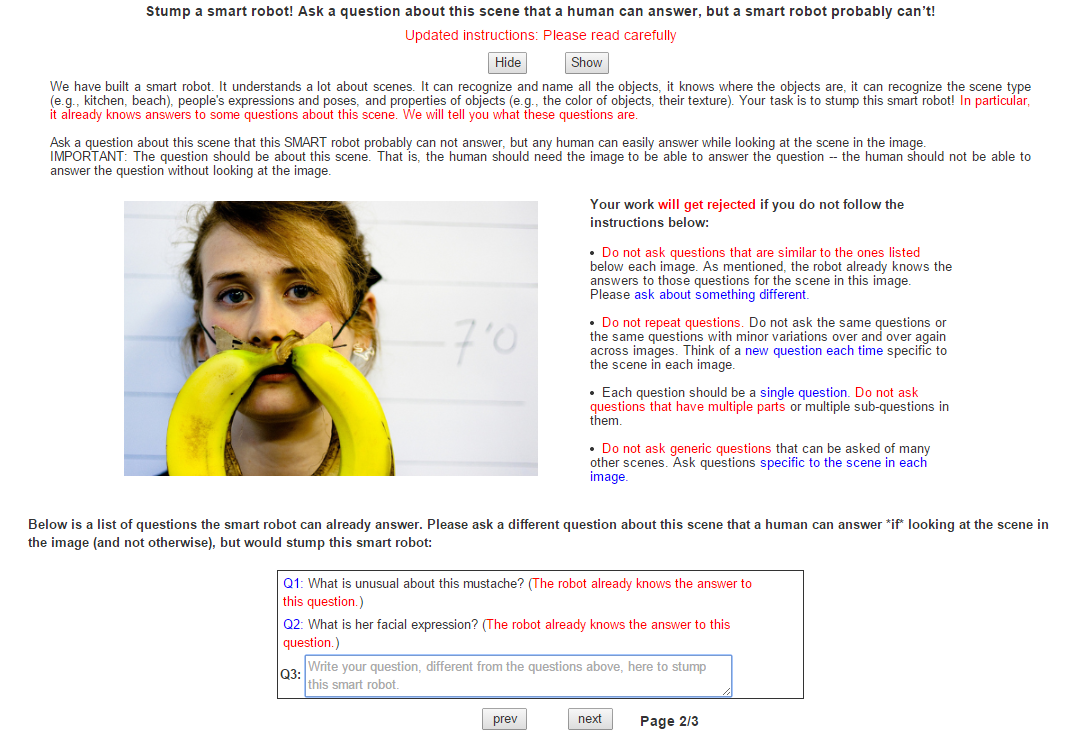
\includegraphics[width=1\linewidth]{figures/question_stage03.png}
\caption{Our AMT interface for collecting the third question for an image, when subjects were shown previous questions that were collected and were asked to ask a question different from previous questions.}
%\vspace{-5pt}
\label{fig:qstage03}
%\setlength{\belowcaptionskip}{-10pt}
\end{figure*}

\begin{figure*}[h]
\centering
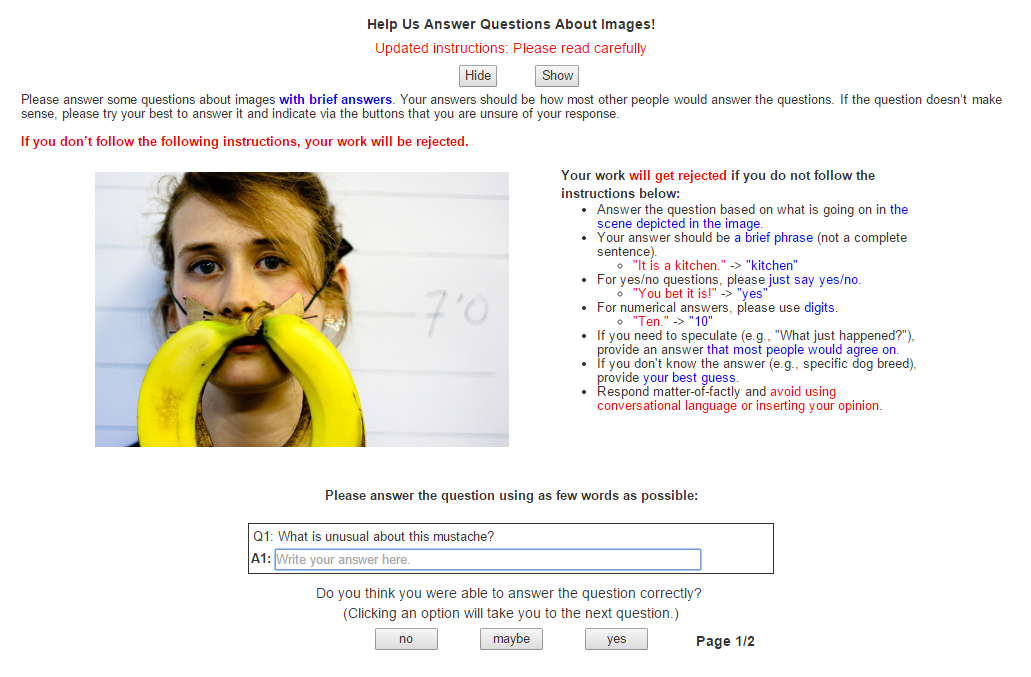
\includegraphics[width=1\linewidth]{figures/answer_with_image.png}
\caption{The AMT interface used to collect answers to a question when subjects were shown the image while answering the question.}
%\vspace{-5pt}
\label{fig:answimage}
%\setlength{\belowcaptionskip}{-10pt}
\end{figure*}

\begin{figure*}[h]
\centering
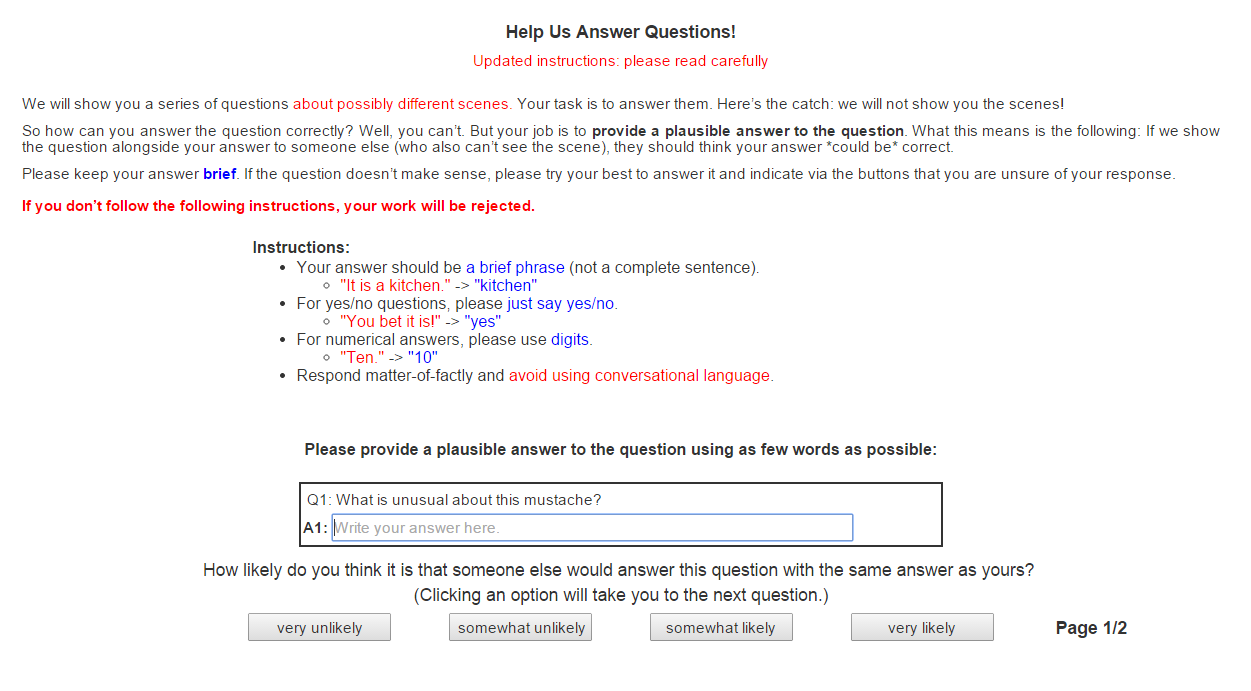
\includegraphics[width=1\linewidth]{figures/answer_without_image.png}
\caption{The AMT interface used to collect answers to a question when subjects were not shown the image while answering the question using only commonsense to collect the plausible, but incorrect, multiple-choice answers.}
%\vspace{-5pt}
\label{fig:answoimage}
%\setlength{\belowcaptionskip}{-10pt}
\end{figure*}
\clearpage

%\vspace{100pt}
\section*{Appendix VIII: Answer Distribution}
\label{sec:top_ans}
\vspace*{-8cm}
The top $250$ answers in our \change{real images} dataset along with their counts and percentage counts are given below. The answers have been presented in different colors to show the different Part-of-Speech (POS) tagging of the answers with the following color code: {\textcolor{magenta}{yes/no}}, {\textcolor{green}{noun}}, {\textcolor{blue}{verb}}, {\textcolor{yellow}{adjective}}, {\textcolor{cyan}{adverb}}, and {\textcolor{red}{numeral}}.

{\textcolor{magenta}{``yes''}} (566613, 22.82\%), {\textcolor{magenta}{``no''}} (381307, 15.35\%), {\textcolor{red}{``2''}} (80031, 3.22\%), {\textcolor{red}{``1''}} (46537, 1.87\%), {\textcolor{yellow}{``white''}} (41753, 1.68\%), {\textcolor{red}{``3''}} (41334, 1.66\%), {\textcolor{yellow}{``red''}} (33834, 1.36\%), {\textcolor{yellow}{``blue''}} (28881, 1.16\%), {\textcolor{red}{``4''}} (27174, 1.09\%), {\textcolor{yellow}{``green''}} (22453, 0.9\%), {\textcolor{yellow}{``black''}} (21852, 0.88\%), {\textcolor{yellow}{``yellow''}} (17312, 0.7\%), {\textcolor{yellow}{``brown''}} (14488, 0.58\%), {\textcolor{red}{``5''}} (14373, 0.58\%), {\textcolor{green}{``tennis''}} (10941, 0.44\%),{\textcolor{green}{``baseball''}} (10299, 0.41\%), {\textcolor{red}{``6''}} (10103, 0.41\%), {\textcolor{green}{``orange''}} (9136, 0.37\%), {\textcolor{red}{``0''}} (8812, 0.35\%), {\textcolor{green}{``bathroom''}} (8473, 0.34\%), {\textcolor{green}{``wood''}} (8219, 0.33\%), {\textcolor{cyan}{``right''}} (8209, 0.33\%), {\textcolor{cyan}{``left''}} (8058, 0.32\%), {\textcolor{green}{``frisbee''}} (7671, 0.31\%), {\textcolor{yellow}{``pink''}} (7519, 0.3\%), {\textcolor{yellow}{``gray''}} (7385, 0.3\%), {\textcolor{green}{``pizza''}} (6892, 0.28\%), {\textcolor{red}{``7''}} (6005, 0.24\%), {\textcolor{green}{``kitchen''}} (5926, 0.24\%), {\textcolor{red}{``8''}} (5592, 0.23\%), {\textcolor{green}{``cat''}} (5514, 0.22\%), {\textcolor{green}{``skiing''}} (5189, 0.21\%), {\textcolor{blue}{``skateboarding''}} (5122, 0.21\%), {\textcolor{green}{``dog''}} (5092, 0.21\%), {\textcolor{green}{``snow''}} (4867, 0.2\%), {\textcolor{yellow}{``black and white''}} (4852, 0.2\%), {\textcolor{green}{``skateboard''}} (4697, 0.19\%), {\textcolor{blue}{``surfing''}} (4544, 0.18\%), {\textcolor{green}{``water''}} (4513, 0.18\%), {\textcolor{green}{``giraffe''}} (4027, 0.16\%), {\textcolor{green}{``grass''}} (3979, 0.16\%), {\textcolor{green}{``surfboard''}} (3934, 0.16\%), {\textcolor{green}{``wii''}} (3898, 0.16\%), {\textcolor{green}{``kite''}} (3852, 0.16\%), {\textcolor{red}{``10''}} (3756, 0.15\%), {\textcolor{yellow}{``purple''}} (3722, 0.15\%), {\textcolor{green}{``elephant''}} (3646, 0.15\%), {\textcolor{green}{``broccoli''}} (3604, 0.15\%), {\textcolor{green}{``man''}} (3590, 0.14\%), {\textcolor{green}{``winter''}} (3490, 0.14\%), {\textcolor{green}{``stop''}} (3413, 0.14\%), {\textcolor{green}{``train''}} (3226, 0.13\%), {\textcolor{red}{``9''}} (3217, 0.13\%), {\textcolor{green}{``apple''}} (3189, 0.13\%), {\textcolor{green}{``silver''}} (3186, 0.13\%), {\textcolor{green}{``horse''}} (3159, 0.13\%), {\textcolor{green}{``banana''}} (3151, 0.13\%), {\textcolor{green}{``umbrella''}} (3139, 0.13\%), {\textcolor{blue}{``eating''}} (3117, 0.13\%), {\textcolor{green}{``sheep''}} (2927, 0.12\%), {\textcolor{green}{``bear''}} (2803, 0.11\%), {\textcolor{green}{``phone''}} (2772, 0.11\%), {\textcolor{red}{``12''}} (2633, 0.11\%), {\textcolor{green}{``motorcycle''}} (2608, 0.11\%), {\textcolor{green}{``cake''}} (2602, 0.1\%), {\textcolor{green}{``wine''}} (2574, 0.1\%), {\textcolor{green}{``beach''}} (2536, 0.1\%), {\textcolor{green}{``soccer''}} (2504, 0.1\%), {\textcolor{yellow}{``sunny''}} (2475, 0.1\%), {\textcolor{green}{``zebra''}} (2403, 0.1\%), {\textcolor{yellow}{``tan''}} (2402, 0.1\%), {\textcolor{green}{``brick''}} (2395, 0.1\%), {\textcolor{green}{``female''}} (2372, 0.1\%), {\textcolor{green}{``bananas''}} (2350, 0.09\%), {\textcolor{green}{``table''}} (2331, 0.09\%), {\textcolor{green}{``laptop''}} (2316, 0.09\%), {\textcolor{green}{``hat''}} (2277, 0.09\%), {\textcolor{green}{``bench''}} (2259, 0.09\%), {\textcolor{green}{``flowers''}} (2219, 0.09\%), {\textcolor{green}{``woman''}} (2197, 0.09\%), {\textcolor{green}{``male''}} (2170, 0.09\%), {\textcolor{green}{``cow''}} (2084, 0.08\%), {\textcolor{green}{``food''}} (2083, 0.08\%), {\textcolor{green}{``living room''}} (2022, 0.08\%), {\textcolor{green}{``bus''}} (2011, 0.08\%), {\textcolor{green}{``snowboarding''}} (1990, 0.08\%), {\textcolor{green}{``kites''}} (1979, 0.08\%), {\textcolor{green}{``cell phone''}} (1943, 0.08\%), {\textcolor{green}{``helmet''}} (1885, 0.08\%), {\textcolor{cyan}{``maybe''}} (1853, 0.07\%), {\textcolor{cyan}{``outside''}} (1846, 0.07\%), {\textcolor{green}{``hot dog''}} (1809, 0.07\%), {\textcolor{green}{``night''}} (1805, 0.07\%), {\textcolor{green}{``trees''}} (1785, 0.07\%), {\textcolor{red}{``11''}} (1753, 0.07\%), {\textcolor{green}{``bird''}} (1739, 0.07\%), {\textcolor{cyan}{``down''}} (1732, 0.07\%), {\textcolor{green}{``bed''}} (1587, 0.06\%), {\textcolor{green}{``camera''}} (1560, 0.06\%), {\textcolor{green}{``tree''}} (1547, 0.06\%), {\textcolor{green}{``christmas''}} (1544, 0.06\%), {\textcolor{green}{``fence''}} (1543, 0.06\%), {\textcolor{green}{``nothing''}} (1538, 0.06\%), {\textcolor{yellow}{``unknown''}} (1532, 0.06\%), {\textcolor{green}{``tennis racket''}} (1525, 0.06\%), {\textcolor{yellow}{``red and white''}} (1518, 0.06\%), {\textcolor{green}{``bedroom''}} (1500, 0.06\%), {\textcolor{green}{``bat''}} (1494, 0.06\%), {\textcolor{green}{``glasses''}} (1491, 0.06\%), {\textcolor{green}{``tile''}} (1487, 0.06\%), {\textcolor{green}{``metal''}} (1470, 0.06\%), {\textcolor{yellow}{``blue and white''}} (1440, 0.06\%), {\textcolor{green}{``fork''}} (1439, 0.06\%), {\textcolor{green}{``plane''}} (1439, 0.06\%), {\textcolor{green}{``airport''}} (1422, 0.06\%), {\textcolor{yellow}{``cloudy''}} (1413, 0.06\%), {\textcolor{red}{``15''}} (1407, 0.06\%), {\textcolor{cyan}{``up''}} (1399, 0.06\%), {\textcolor{yellow}{``blonde''}} (1398, 0.06\%), {\textcolor{green}{``day''}} (1396, 0.06\%), {\textcolor{green}{``teddy bear''}} (1386, 0.06\%), {\textcolor{green}{``glass''}} (1379, 0.06\%), {\textcolor{red}{``20''}} (1365, 0.05\%), {\textcolor{green}{``beer''}} (1345, 0.05\%), {\textcolor{green}{``car''}} (1331, 0.05\%), {\textcolor{blue}{``sitting''}} (1328, 0.05\%), {\textcolor{green}{``boat''}} (1326, 0.05\%), {\textcolor{blue}{``standing''}} (1326, 0.05\%), {\textcolor{yellow}{``clear''}} (1318, 0.05\%), {\textcolor{red}{``13''}} (1318, 0.05\%), {\textcolor{green}{``nike''}} (1293, 0.05\%), {\textcolor{green}{``sand''}} (1282, 0.05\%), {\textcolor{yellow}{``open''}} (1279, 0.05\%), {\textcolor{green}{``cows''}} (1271, 0.05\%), {\textcolor{green}{``bike''}} (1267, 0.05\%), {\textcolor{green}{``chocolate''}} (1266, 0.05\%), {\textcolor{green}{``donut''}} (1263, 0.05\%), {\textcolor{green}{``airplane''}} (1247, 0.05\%), {\textcolor{green}{``birthday''}} (1241, 0.05\%), {\textcolor{green}{``carrots''}} (1239, 0.05\%), {\textcolor{green}{``skis''}} (1220, 0.05\%), {\textcolor{green}{``girl''}} (1220, 0.05\%), {\textcolor{yellow}{``many''}} (1211, 0.05\%), {\textcolor{green}{``zoo''}} (1204, 0.05\%), {\textcolor{green}{``suitcase''}} (1199, 0.05\%), {\textcolor{yellow}{``old''}} (1180, 0.05\%), {\textcolor{green}{``chair''}} (1174, 0.05\%), {\textcolor{yellow}{``beige''}} (1170, 0.05\%), {\textcolor{green}{``ball''}} (1169, 0.05\%), {\textcolor{green}{``ocean''}} (1168, 0.05\%), {\textcolor{green}{``sandwich''}} (1168, 0.05\%), {\textcolor{green}{``tie''}} (1166, 0.05\%), {\textcolor{green}{``horses''}} (1163, 0.05\%), {\textcolor{green}{``palm''}} (1163, 0.05\%), {\textcolor{green}{``stripes''}} (1155, 0.05\%), {\textcolor{green}{``fall''}} (1146, 0.05\%), {\textcolor{green}{``cheese''}} (1142, 0.05\%), {\textcolor{green}{``scissors''}} (1134, 0.05\%), {\textcolor{green}{``round''}} (1125, 0.05\%), {\textcolor{yellow}{``chinese''}} (1123, 0.05\%), {\textcolor{green}{``knife''}} (1120, 0.05\%), {\textcolor{red}{``14''}} (1110, 0.04\%), {\textcolor{green}{``toilet''}} (1099, 0.04\%), {\textcolor{blue}{``don't know''}} (1085, 0.04\%), {\textcolor{green}{``snowboard''}} (1083, 0.04\%), {\textcolor{green}{``truck''}} (1076, 0.04\%), {\textcolor{green}{``boy''}} (1070, 0.04\%), {\textcolor{green}{``coffee''}} (1070, 0.04\%), {\textcolor{yellow}{``cold''}} (1064, 0.04\%), {\textcolor{green}{``fruit''}} (1064, 0.04\%), {\textcolor{blue}{``walking''}} (1053, 0.04\%), {\textcolor{green}{``wedding''}} (1051, 0.04\%), {\textcolor{green}{``lot''}} (1050, 0.04\%), {\textcolor{green}{``sunglasses''}} (1047, 0.04\%), {\textcolor{green}{``mountains''}} (1030, 0.04\%), {\textcolor{green}{``wall''}} (1009, 0.04\%), {\textcolor{green}{``elephants''}} (1006, 0.04\%), {\textcolor{green}{``wetsuit''}} (998, 0.04\%), {\textcolor{green}{``square''}} (994, 0.04\%), {\textcolor{green}{``toothbrush''}} (989, 0.04\%), {\textcolor{blue}{``sleeping''}} (986, 0.04\%), {\textcolor{green}{``fire hydrant''}} (977, 0.04\%), {\textcolor{green}{``bicycle''}} (973, 0.04\%), {\textcolor{green}{``overcast''}} (968, 0.04\%), {\textcolor{green}{``donuts''}} (961, 0.04\%), {\textcolor{green}{``plastic''}} (961, 0.04\%), {\textcolor{green}{``breakfast''}} (955, 0.04\%), {\textcolor{green}{``tv''}} (953, 0.04\%), {\textcolor{green}{``paper''}} (952, 0.04\%), {\textcolor{green}{``ground''}} (949, 0.04\%), {\textcolor{yellow}{``asian''}} (938, 0.04\%), {\textcolor{green}{``plaid''}} (936, 0.04\%), {\textcolor{green}{``dirt''}} (933, 0.04\%), {\textcolor{green}{``mirror''}} (928, 0.04\%), {\textcolor{green}{``usa''}} (928, 0.04\%), {\textcolor{green}{``chicken''}} (925, 0.04\%), {\textcolor{green}{``plate''}} (920, 0.04\%), {\textcolor{green}{``clock''}} (912, 0.04\%), {\textcolor{green}{``luggage''}} (908, 0.04\%), {\textcolor{green}{``none''}} (908, 0.04\%), {\textcolor{green}{``street''}} (905, 0.04\%), {\textcolor{cyan}{``on table''}} (904, 0.04\%), {\textcolor{green}{``spoon''}} (899, 0.04\%), {\textcolor{blue}{``cooking''}} (898, 0.04\%), {\textcolor{yellow}{``daytime''}} (896, 0.04\%), {\textcolor{red}{``16''}} (893, 0.04\%), {\textcolor{green}{``africa''}} (890, 0.04\%), {\textcolor{green}{``stone''}} (884, 0.04\%), {\textcolor{yellow}{``not sure''}} (873, 0.04\%), {\textcolor{green}{``window''}} (868, 0.03\%), {\textcolor{green}{``sun''}} (865, 0.03\%), {\textcolor{green}{``gold''}} (860, 0.03\%), {\textcolor{green}{``people''}} (856, 0.03\%), {\textcolor{green}{``racket''}} (847, 0.03\%), {\textcolor{green}{``zebras''}} (845, 0.03\%), {\textcolor{green}{``carrot''}} (841, 0.03\%), {\textcolor{green}{``person''}} (835, 0.03\%), {\textcolor{green}{``fish''}} (835, 0.03\%), {\textcolor{yellow}{``happy''}} (824, 0.03\%), {\textcolor{green}{``circle''}} (822, 0.03\%), {\textcolor{green}{``oranges''}} (817, 0.03\%), {\textcolor{green}{``backpack''}} (812, 0.03\%), {\textcolor{red}{``25''}} (810, 0.03\%), {\textcolor{green}{``leaves''}} (809, 0.03\%), {\textcolor{green}{``watch''}} (804, 0.03\%), {\textcolor{green}{``mountain''}} (800, 0.03\%), {\textcolor{green}{``no one''}} (798, 0.03\%), {\textcolor{green}{``ski poles''}} (792, 0.03\%), {\textcolor{green}{``city''}} (791, 0.03\%), {\textcolor{green}{``couch''}} (790, 0.03\%), {\textcolor{green}{``afternoon''}} (782, 0.03\%), {\textcolor{green}{``jeans''}} (781, 0.03\%), {\textcolor{yellow}{``brown and white''}} (779, 0.03\%), {\textcolor{green}{``summer''}} (774, 0.03\%), {\textcolor{green}{``giraffes''}} (772, 0.03\%), {\textcolor{green}{``computer''}} (771, 0.03\%), {\textcolor{green}{``refrigerator''}} (768, 0.03\%), {\textcolor{green}{``birds''}} (762, 0.03\%), {\textcolor{green}{``child''}} (761, 0.03\%), {\textcolor{green}{``park''}} (759, 0.03\%), {\textcolor{blue}{``flying kite''}} (756, 0.03\%), {\textcolor{green}{``restaurant''}} (747, 0.03\%), {\textcolor{green}{``evening''}} (738, 0.03\%), {\textcolor{green}{``graffiti''}} (736, 0.03\%), {\textcolor{red}{``30''}} (730, 0.03\%), {\textcolor{blue}{``grazing''}} (727, 0.03\%), {\textcolor{green}{``flower''}} (723, 0.03\%), {\textcolor{yellow}{``remote''}} (720, 0.03\%), {\textcolor{green}{``hay''}} (719, 0.03\%), {\textcolor{red}{``50''}} (716, 0.03\%). 


\section*{Appendix IX: Additional Examples}
\label{sec:dataset_stats}

To provide insight into the dataset, we provide additional examples. In \figref{fig:coco_more_examples}, \figref{fig:abstract_more_examples}, and \figref{fig:mc_examples}, we show a random selection of the VQA dataset for the MS COCO~\cite{coco} images, abstract scenes, and multiple-choice questions, respectively.

\begin{figure*}[t]
\centering
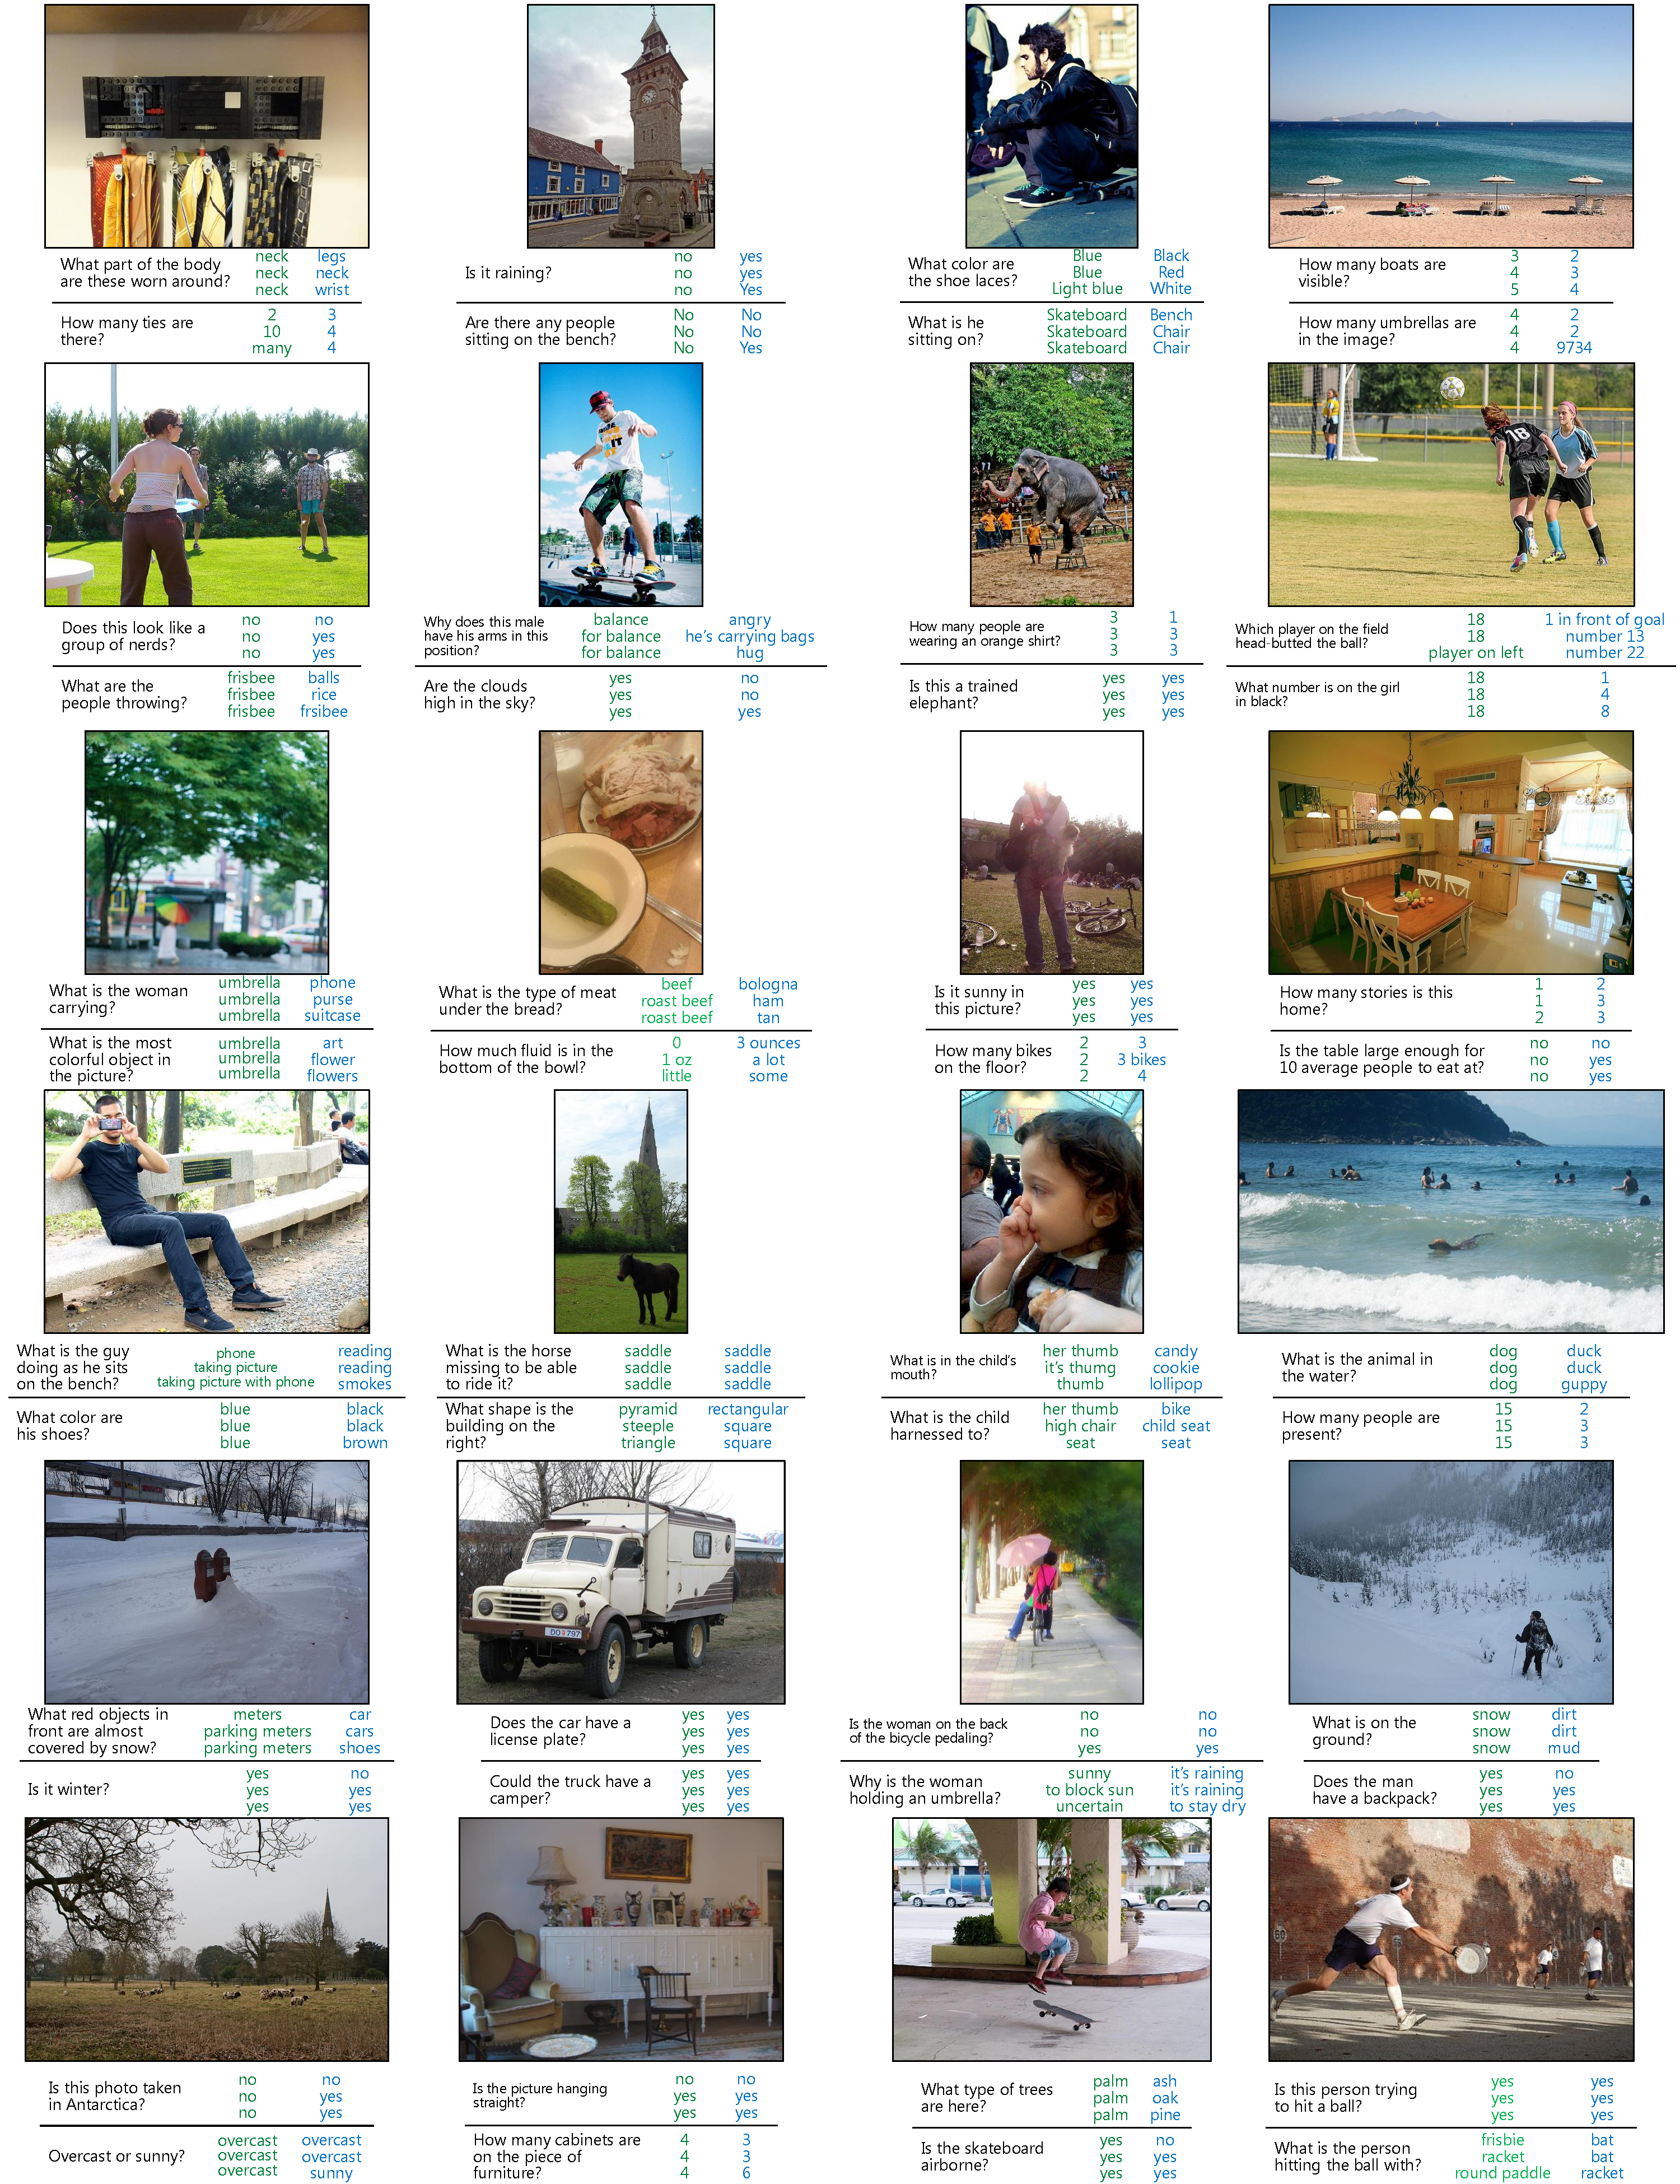
\includegraphics[width=1\linewidth]{figures/coco_examples-compressed.pdf}
\caption{Random examples of questions (black), \change{(a subset of the)} answers given when looking at the image (green), and answers given when not looking at the image (blue) for numerous representative examples of the real image dataset.}
%\vspace{-5pt}
\label{fig:coco_more_examples}
%\setlength{\belowcaptionskip}{-10pt}
\end{figure*}

\begin{figure*}[t]
\centering
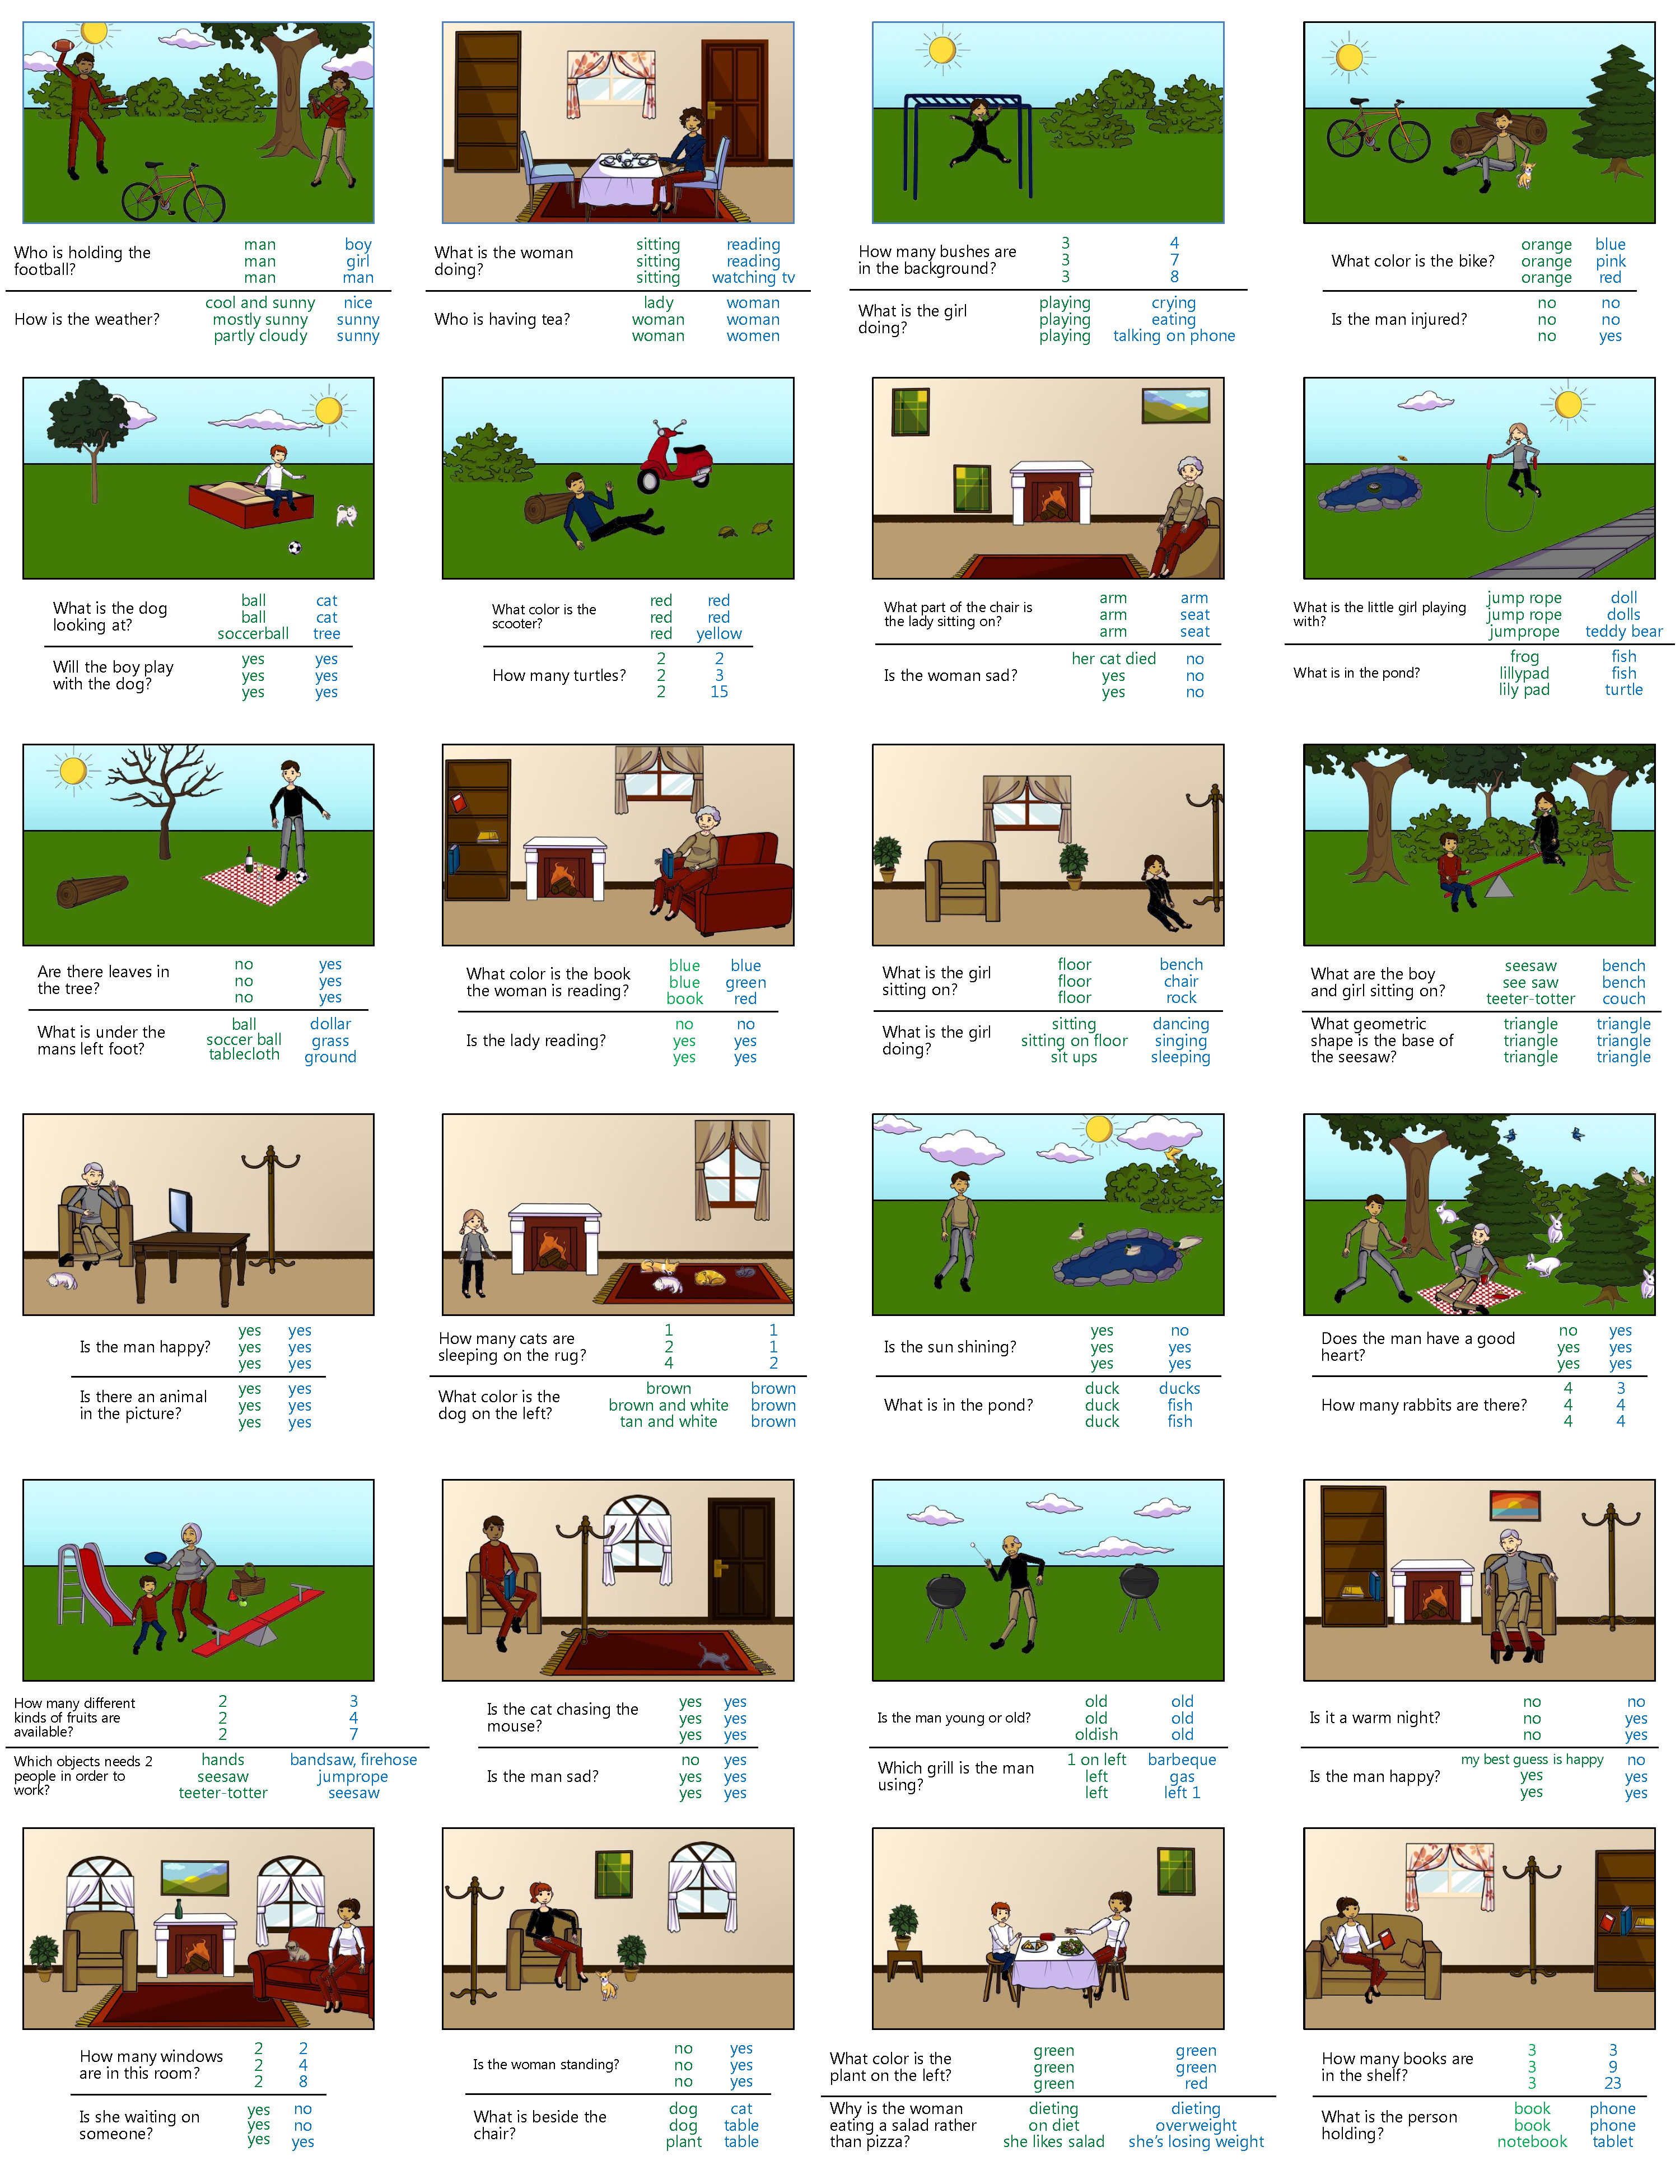
\includegraphics[width=1\linewidth]{figures/abstract_examples-compressed.pdf}
\caption{Random examples of questions (black), \change{(a subset of the)} answers given when looking at the image (green), and answers given when not looking at the image (blue) for numerous representative examples of the abstract scene dataset.}
%\vspace{-5pt}
\label{fig:abstract_more_examples}
%\setlength{\belowcaptionskip}{-10pt}
\end{figure*}

\begin{figure*}[t]
\centering
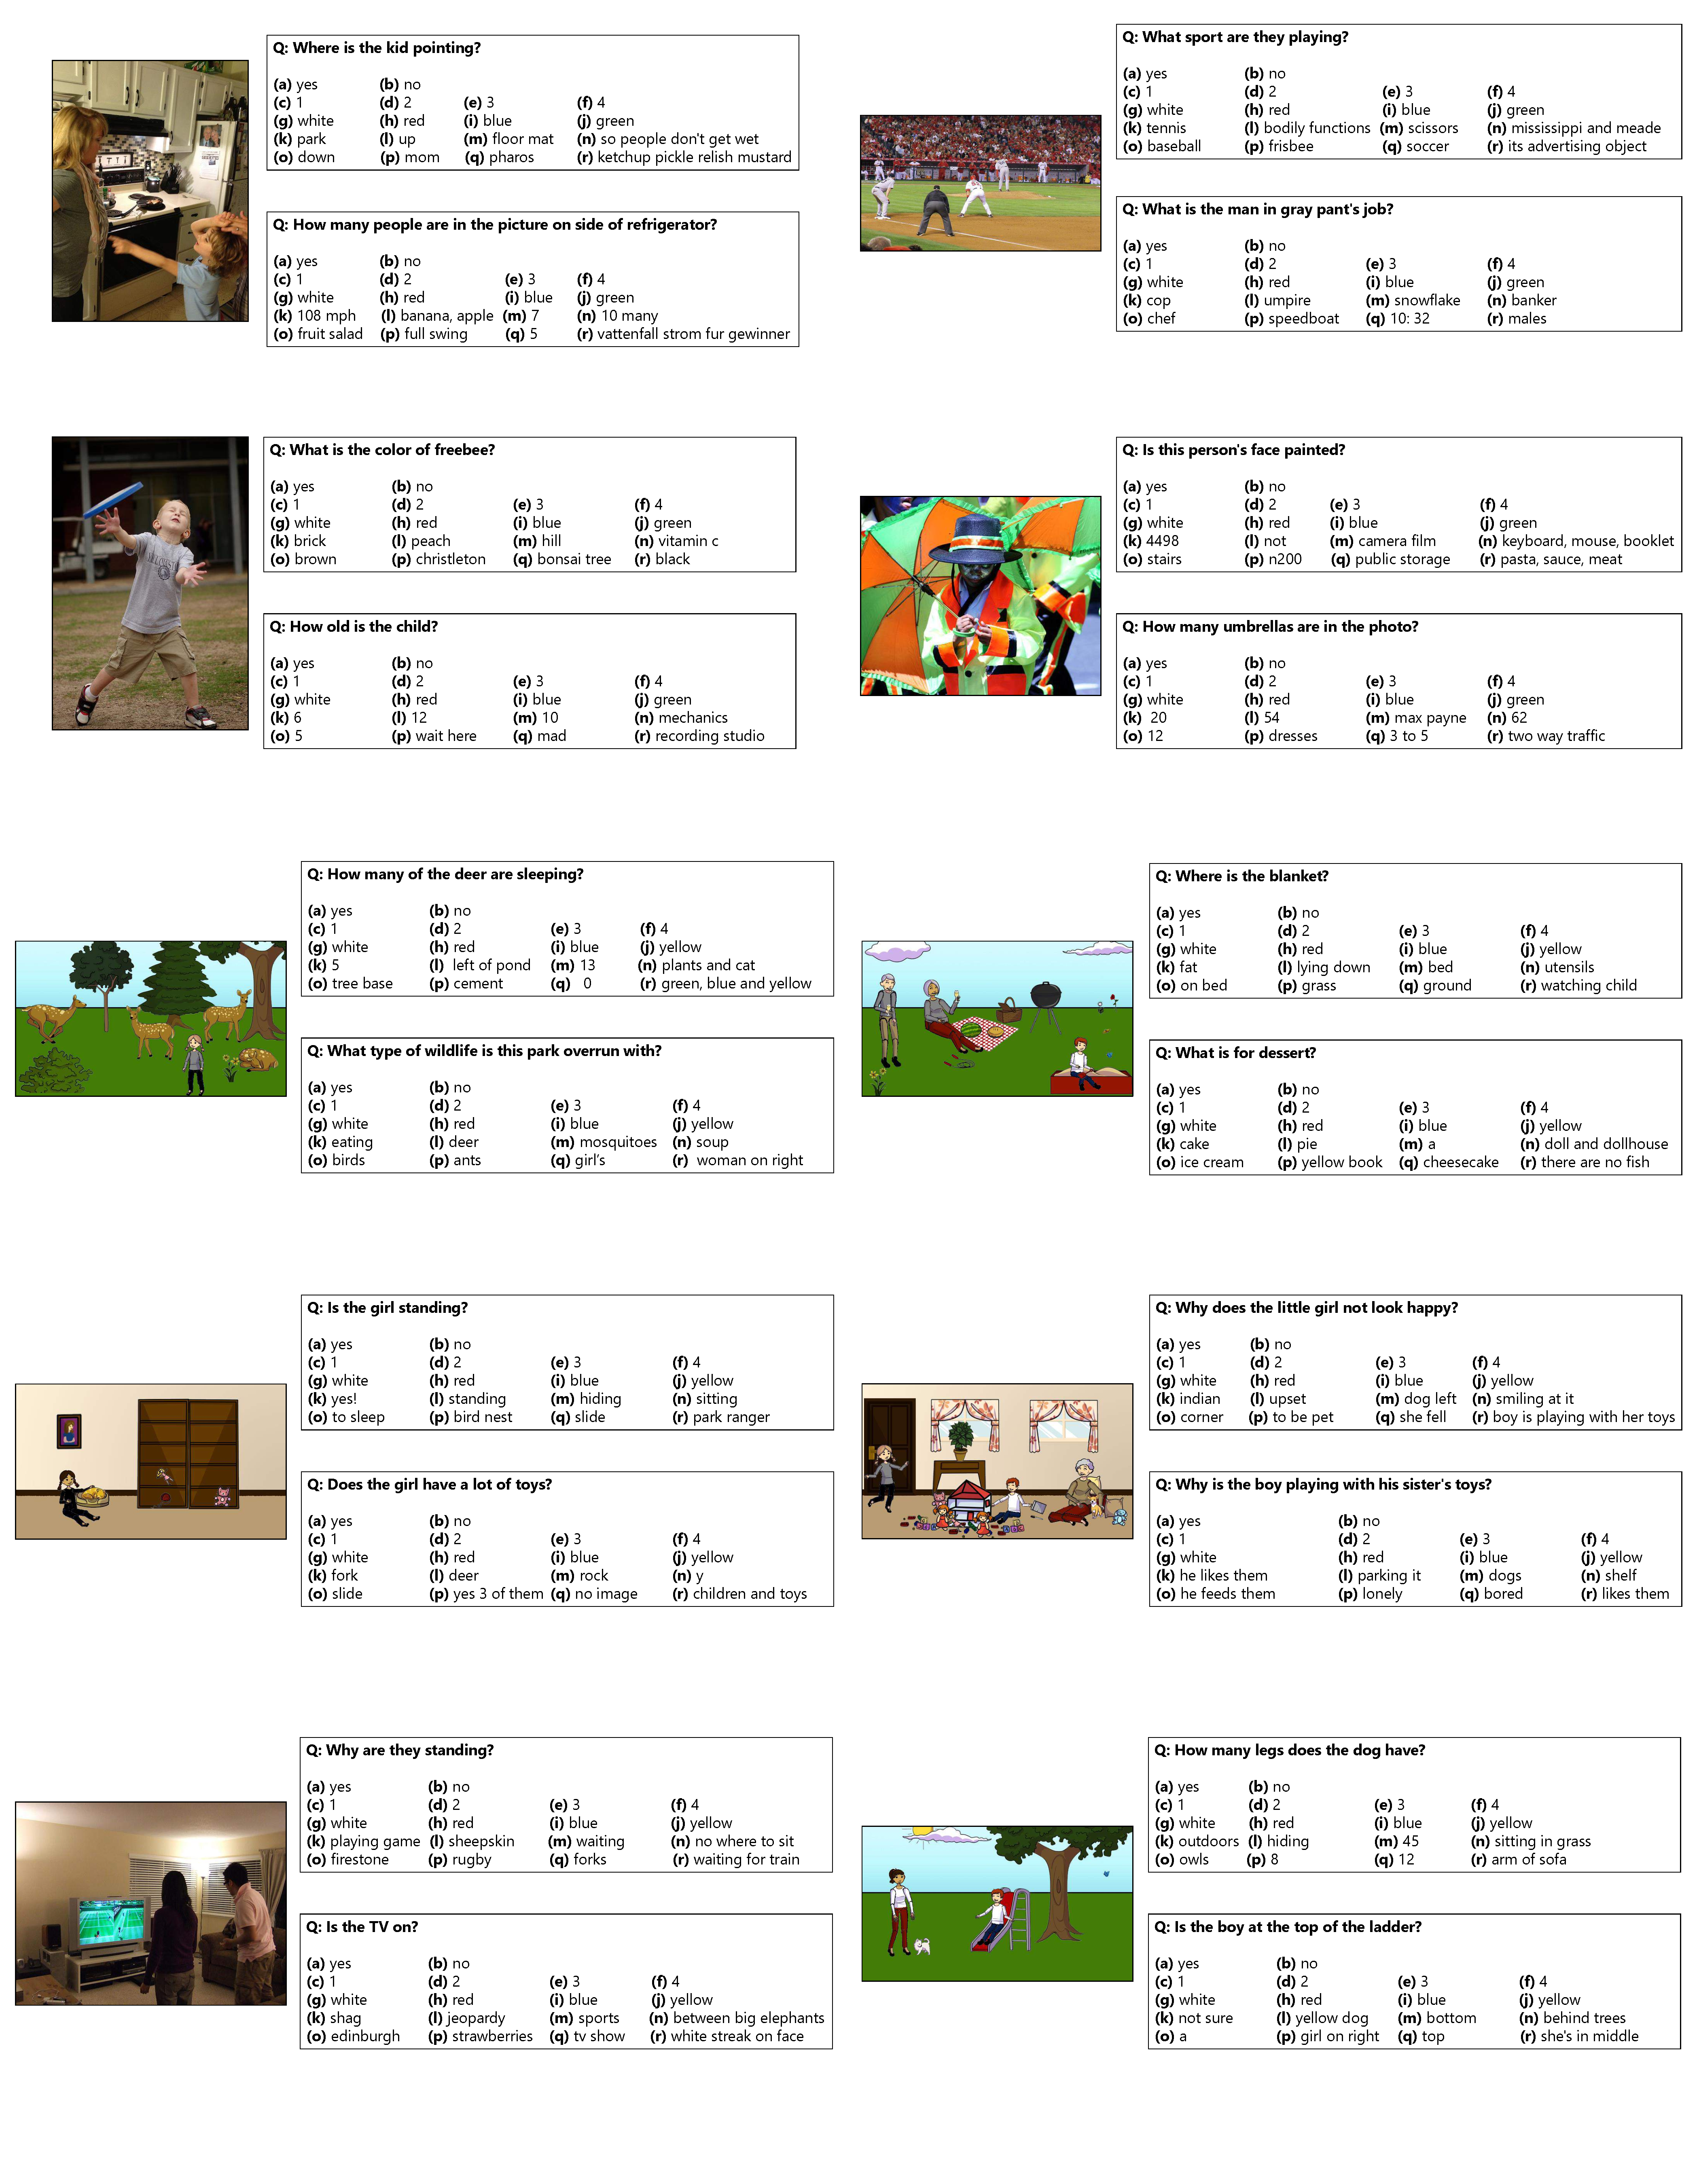
\includegraphics[width=1\linewidth]{figures/MC_examples_compressed.pdf}
\caption{Random examples of multiple-choice questions for numerous representative examples of the real and abstract scene dataset.}
%\vspace{-5pt}
\label{fig:mc_examples}
%\setlength{\belowcaptionskip}{-10pt}
\end{figure*}